\documentclass[a4paper,11pt]{book}

\setcounter{tocdepth}{3}
\setcounter{secnumdepth}{3}




%%%%%%%%%%%%%%%%%%%%%%%%% GEOMETRY %%%%%%%%%%%%%%%%%%%%%%%%%%%%

%\usepackage[top=Bcm, bottom=Hcm, outer=Ccm, inner=Acm, heightrounded, marginparwidth=Ecm, marginparsep=Dcm]{geometry}		
\usepackage[outer=5cm, heightrounded, marginparwidth=4cm, marginparsep=0.5cm]{geometry}														
																																										
%%%%%%%%%%%%%%%%%%%%%%% Document Setup %%%%%%%%%%%%%%%%%%%%%%%%%%%%

\usepackage[T1]{fontenc} 		% to get Type 1 fonts
\usepackage[utf8]{inputenc} 	% to enable non ASCII characters
\usepackage{lmodern}
\usepackage[english]{babel}
\usepackage{quotchap}
\usepackage{marginnote}
\usepackage{xcolor}
\usepackage{xargs}     			% Use more than one optional parameter in a new commands
\usepackage{ragged2e}
\usepackage{setspace}
\usepackage{calc}				%Adds in­fix ex­pres­sions to per­form arith­metic on the ar­gu­ments of the LATEX com­mands \set­counter, 
									%\ad­dto­counter, \setlength, and \ad­dtolength. 
\usepackage{calculator}
\usepackage{hyphenat}		%prevent hyphenation
\usepackage{twoopt}			%Create commands with two optional arguments

\usepackage[titletoc,title]{appendix}
\usepackage{imakeidx} 
\usepackage{cleveref}
\usepackage{hyperref}

\hypersetup{
    colorlinks,
    citecolor=black,
    filecolor=black,
    linkcolor=black,
    urlcolor=black
}

%%%%%%%%%%%%%%%%%%%%%%%%%% Columns, tables, and Lists %%%%%%%%%%%%%%%%%%%%%%%
\usepackage{multicol}
\usepackage{tabu}
\usepackage{tabularx}
\usepackage{enumitem}
\usepackage{stackengine}		%pro­vides a ver­sa­tile way to stack ob­jects ver­ti­cally in a va­ri­ety of cus­tomiz­able ways

%%%%%%%%%%%%%%%%%%%%%%%%%%%%%% Boxes %%%%%%%%%%%%%%%%%%%%%%%%%%%%
\usepackage{float}				%Im­proves the in­ter­face for defin­ing float­ing ob­jects such as fig­ures and ta­bles
\usepackage[export]{adjustbox}
\usepackage{mdframed}
\usepackage{changepage}

\usepackage[most,breakable,many]{tcolorbox}
\tcbset{before skip=0pt,after skip=0pt} 


%%%%%%%%%%%%%%%%%%%%%%%%%%%%%% Verbatim and Dummy Text %%%%%%%%%%%%%%%%%%%
\usepackage{lipsum}			% dummy text
\usepackage{verbatim}
\usepackage{fancyvrb}
\usepackage{listings}


%%%%%%%%%%%%%%%%%%%%%%%%%%%%%% Graphing %%%%%%%%%%%%%%%%%%%%%%%%%%%

\usepackage{standalone}		%allows users to easily place picture environments or other material in own source 
									%files and compile these on their own or as part of a main document
\usepackage{graphicx}			%figure handler
\usepackage{wrapfig}			%wrap figures
\usepackage{caption}
\usepackage{subcaption}
\usepackage{transparent}
\usepackage{pgfplots}
%\usetikzlibrary{positioning}
\usepackage{tikz}

%%%%%%%%%%%%%%%%%%%%%%% Math Symbols %%%%%%%%%%%%%%%%%%%%%%%%%%%%%%%%

\usepackage{mathtools}		%use math environments
\usepackage{amssymb}  		%use math symbols
\usepackage{amsthm}		
\usepackage{amsmath}
\usepackage{cancel}			%cross out terms
\usepackage{gensymb}	    		% to use the degree symbol
\usepackage{eucal}        		% Caligraphy style font
\usepackage{mathrsfs}     		% script style font
\usepackage{esint}				%cyclic integral
\usepackage{MnSymbol}

%%%%%%%%%%%%%%%%%%%%%%%% UNITS %%%%%%%%%%%%%%%%%%%%%%%%%%%%%%%%%%
													
\usepackage{siunitx}																	
																							
  \let\DeclareUSUnit\DeclareSIUnit													
  \let\US\SI																				
																							
  %length units																			
  \DeclareUSUnit\inch{in}													
  \DeclareUSUnit\feet{ft}																
  \DeclareUSUnit\yard{yd}																
  \DeclareUSUnit\mile{mi}																
																							
  %Volume units																			
  \DeclareUSUnit\floz{fl oz}																
  \DeclareUSUnit\gallon{gal}					

  %Surface units		
  \DeclareSIUnit\are{a}	
  \DeclareUSUnit\acre{ac}		
																							
  %Temperature Units																	
  \DeclareUSUnit\fahrenheit{\SIUnitSymbolDegree F}								
																							
  %Mass units																			
  \DeclareUSUnit\ton{ton}																
  \DeclareUSUnit\pound{lb}															
																							
  %Pressure units																		
  \DeclareUSUnit\torr{torr}																
  \DeclareUSUnit\mmHg{mmHg}														
  \DeclareUSUnit\atm{atm}															
  \DeclareUSUnit\bar{bar}																
  \DeclareUSUnit\psi{psi}																

%%%%%%%%%%%%%%%%%%%%%%%%%%%% Margin Note %%%%%%%%%%%%%%%%%%%%%%%%%%%%
\newcommand*\mnote[3][0pt]{%
  \if l#2\reversemarginpar\def\pointer{\filledmedtriangleright}%
    \def\stackalignment{r}\fi%
  \if r#2\normalmarginpar\def\pointer{\filledmedtriangleleft}%
    \def\stackalignment{l}\fi%
  \marginpar{%
    \topinset{%
      \scalebox{1.5}{\textcolor{blue}{$\pointer$}}}{%
      \belowbaseline[-1.5\baselineskip-#1]{%
        \stackengine%
          {-5pt}%
          {\fcolorbox{blue}{white}{\parbox{1.8cm}%
            {\vspace{3pt}\raggedright#3}}}%
          {~\colorbox{white}{\sffamily Note}}%
          {O}%
          {l}%
          {F}%
          {F}%
          {S}%
        }%
      }{%
      3ex+#1}{%
      -2ex}%
  }%
}

%%%%%%%%%%%%%%%%%%%%%%%%% Defining a frame %%%%%%%%%%%%%%%%%%%%%%%%%%%%%

\mdfdefinestyle{MyFrame}{%
    %linecolor=blue,
    outerlinewidth=3pt,
    roundcorner=10pt,
    innertopmargin=\baselineskip,
    innerbottommargin=\baselineskip,
    innerrightmargin=20pt,
    innerleftmargin=20pt,
    %backgroundcolor=gray!50!white
    }

%%%%%%%%%%%%%%%%%%%%%%%%%% Useful short Commands %%%%%%%%%%%%%%%%%%%%%%%%%


\newcommand{\EMPH}[1]{\textit{#1}}
\newcommandtwoopt{\magn}[3][][]{\left|\vec{#3}^{#2}_{\textit{\tiny #1}} \right|}		% Magnitude of a vector: 1st command is the subindex, 2nd the superindex, third the vector
\newcommand{\der}[2]{\frac{d}{d#2}\left(#1\right)}								% Derivative
\newcommand{\nder}[3]{\frac{d^{#3}}{d#2^{#3}}\left(#1\right)}			% Nth Derivative
\newcommand{\pder}[2]{\frac{\partial}{\partial#2}\left(#1\right)}				% Partial Derivative
\newcommand{\npder}[3]{\frac{\partial^{#3}}{\partial#2^{#3}}\left(#1\right)}%Nth Partial Derivative

\newcommand{\modulo}[2]{%
  \FPeval{\result}{trunc(#1-(#2*trunc(#1/#2,0)),0)}\result%
}

%%%%%%%%%%%%%%%%%%%%%%%%%% dummy text by lines %%%%%%%%%%%%%%%%%%%%%%%%%%
\newbox\one																																																
\newbox\two																																																
\long\def\loremlines#1{%																																												
    \setbox\one=\vbox {%																																														
      \lipsum																																						
     }%																																																		
   \setbox\two=\vsplit\one to #1\baselineskip%																																					
   \unvbox\two}%																																														


%%%%%%%%%%%%%%%%%%%%%%%%%%% Objectives %%%%%%%%%%%%%%%%%%%%%%%%%%%%%%								
																																								
\newtcolorbox{objbox}[1]{colback=red!5!white,colframe=red!75!black,fonttitle=\bfseries,title=#1}	%							
\newenvironment{objectives}{%																														
	\begin{objbox}{Objectives:} \begin{list}{\(\bullet\)}{}%																					
}{%																																							
	\end{list} \end{objbox}%																															
}%																																							
																																								
%%%%%%%%%%%%%%%%%%%%%%%%%% Some Theorems %%%%%%%%%%%%%%%%%%%%%%%%%%%%
%\newtheorem{definition}{Definition}																												
%\newtheorem{example}{Example}																												
\newtheorem{case}{Real Life Example}																											
																																								
																																								
%%%%%%%%%%%%%%%%%%%%%%%%%% Definition %%%%%%%%%%%%%%%%%%%%%%%%%%%%%%%
\newtcbtheorem[number within=chapter]{definition}{Definition}%																		
{colback=green!5,colframe=green!35!black,fonttitle=\bfseries}{th}%																	
																																								
%%%%%%%%%%%%%%%%%%%%%%%%%% Description %%%%%%%%%%%%%%%%%%%%%%%%%%%%%%								
\newlist{Description}{description}{3}%																											
\setlist[Description]{style=nextline}%																												
\SetEnumitemKey{margin}{leftmargin={\widthof{#1}+2em}}%																			
																																								
%%%%%%%%%%%%%%%%%%%%%%%%%% Example %%%%%%%%%%%%%%%%%%%%%%%%%%%%%%%
																									
\newtcbtheorem[number within=section]{example}{Example}%																			
{colback=blue!5,colframe=blue!35!black,fonttitle=\bfseries, before skip=5pt,after skip=10pt,righttitle=\linewidth}{th}%																		


%%%%%%%%%%%%%%%%%%%%%%%%%% Exercise %%%%%%%%%%%%%%%%%%%%%%%%%%%%%%%
																									
\newtcbtheorem[number within=section]{exercise}{Exercise}%																			
{colback=blue!5,colframe=blue!35!black,fonttitle=\bfseries, before skip=5pt,after skip=10pt}{th}%																		
																																								
%%%%%%%%%%%%%%%%%%%%%%%%%% Hint Note %%%%%%%%%%%%%%%%%%%%%%%%%%%%%%%
											
\newcounter{hint}																																		
\newtcolorbox[use counter=hint]																														
  {hint}[1][]																																				
  {title=Hint~\thetcbcounter,																															
   width=4cm,																																				
   left=0pt,																																					
   right=0pt,																																				
   fonttitle=\bfseries\color{white},																													
   colframe=orange,																																		
   colback=orange!10,																																	
   #1																																							
}   																																							
\newcommand\Hint[3][]{%																															
  \marginnote[#1]{%																																	
    \makebox[0pt][l]{\begin{hint}[label=#3]																										
    #2																																							
    \end{hint}}}}%																																		
    																																							
%%%%%%%%%%%%%%%%%%%%%%%%% Important Note %%%%%%%%%%%%%%%%%%%%%%%%%%%%%%
										
\newcounter{important}                                                                                                                              
\newtcolorbox[use counter=important]                                                                                                                
{important}[1][]                                                                                                                                          
{title=Important Note~\thetcbcounter, 
  center title,                                                                                                        
  width=4cm,                                                                                                                                               
  left=0pt,                                                                                                                                                    
  right=0pt,                                                                                                                                               
  fonttitle=\bfseries\color{black},                                                                                                                    
  colframe=orange,                                                                                                                                      
  colback=orange!10,                                                                                                                                        
  #1                                                                                                                                                           
}                                                                                                                                                               

\newcommand{\isimportant}[3][]{%
  \ifodd\value{page}
  \marginnote{%
    \makebox[0pt][l]{%
      \begin{important}[label=#3]
        #2%
      \end{important}%
    }%
  }[\ifblank{#1}{0pt}{#1}]%
  \else
  \marginnote[%
  {%
    \makebox[0pt][r]{%
      \begin{important}[label=#3]%
        #2%
      \end{important}
    }%
  }]{}[\ifblank{#1}{0pt}{#1}]%
  \fi
}
%%%%%%%%%%%%%%%%%%%%%%%%% Remember Note %%%%%%%%%%%%%%%%%%%%%%%%%%%%%%
										
\newcounter{remember}																																
\newtcolorbox[use counter=remember]																												
  {remember}[1][]																																			
  {title=Remember ~\thetcbcounter,																											
   width=4cm,																																				
   left=0pt,																																					
   right=0pt,																																				
   fonttitle=\bfseries\color{white},																													
   colframe=violet,																																		
   colback=violet!10,																																		
   #1																																							
}   																																							
\newcommand\Remember[3][]{%																													
  \marginnote[#1]{%																																	
    \makebox[0pt][l]{\begin{remember}[label=#3]																								
    #2																																							
    \end{remember}}}}%	

%%%%%%%%%%%%%%%%%%%%%%%%% Todo Notes %%%%%%%%%%%%%%%%%%%%%%%%%%%%%%
\newcommandx{\unsure}[2][1=]{\todo[linecolor=red,backgroundcolor=red!25,bordercolor=red,#1]{#2}}
\newcommandx{\change}[2][1=]{\todo[linecolor=blue,backgroundcolor=blue!25,bordercolor=blue,#1]{#2}}
\newcommandx{\info}[2][1=]{\todo[linecolor=OliveGreen,backgroundcolor=OliveGreen!25,bordercolor=OliveGreen,#1]{#2}}
\newcommandx{\improvement}[2][1=]{\todo[linecolor=Plum,backgroundcolor=Plum!25,bordercolor=Plum,#1]{#2}}
\newcommandx{\thiswillnotshow}[2][1=]{\todo[disable,#1]{#2}}																															
    																																							
%%%%%%%%%%%%%%%%%%%%%%%%% Common abbreviations %%%%%%%%%%%%%%%%%%%%%%%%%%%


\newcommand{\etal}{\textit{et al}. }
\newcommand{\ie}{\textit{i}.\textit{e}. }
\newcommand{\eg}{\textit{e}.\textit{g}. }
\newcommand{\Index}[1]{\index{#1}\nohyphens{\textbf{\textsc{#1}}}}

\newcommand{\command}[1]{\texttt{\string#1}}
\newcommand{\sub}[2]{#1^{}_{\textnormal{\tiny #2}}\ }		%smaller subindex
%%%%%%%%%%%%%%%%%%%%%%%%% Columns with equations %%%%%%%%%%%%%%%%%%%%%%%%%%%

\newcolumntype{C}{>{$}c<{$}}
\newcolumntype{L}{>{$}l<{$}}
\newcolumntype{R}{>{$}r<{$}}

\newcolumntype{E}{>{\begin{minipage}{5cm}\begin{equation*}}c<{\end{equation*}\end{minipage}}}
																													
%%%%%%%%%%%%%%%%%%%%%%%%%%%%%%%%%%%%%%%%%%%%%%%%
% Chapter quote at the start of chapter        %
% Source: http://tex.stackexchange.com/a/53380 %
%%%%%%%%%%%%%%%%%%%%%%%%%%%%%%%%%%%%%%%%%%%%%%%%%%%%
\makeatletter
\renewcommand{\@chapapp}{}% Not necessary...
\newenvironment{chapquote}[2][2em]
  {\setlength{\@tempdima}{#1}%
   \def\chapquote@author{#2}%
   \parshape 1 \@tempdima \dimexpr\textwidth-2\@tempdima\relax%
   \itshape}
  {\par\normalfont\hfill--\ \chapquote@author\hspace*{\@tempdima}\par\bigskip}
\makeatother

%%%%%%%%%%%%%%%%%%%%%%%%%%%%%%%%%%%%%%%%%%%%%%%%%%%%

\newcommand\numberthis{\addtocounter{equation}{1}\tag{\theequation}}

%%%%%%%%%%%%%%%%%%%%%%%%%%%%%%%%%%%%%%%%%%%%%%%%%%%%

\renewcommand{\vec}[1]{\mathbf{#1}}	%changes vectors to boldtype
\let\oldhat\hat
%\renewcommand{\hat}[1]{\oldhat{\mathbf{#1}}}
\renewcommand{\hat}[1]{\boldsymbol{\oldhat{\mathbf{#1}}}}
\newcommand{\ihat}{\hat{\textbf{\i}}}
\newcommand{\jhat}{\hat{\textbf{\j}}}
\newcommand{\khat}{\hat{\textbf{k}}}



\begin{comment}
%%%%%%%%%%%%%%%%%%%%Questions%%%%%%%%%%%%%%%%%%%%%
\makeatletter
\newcommand{\printquestions}{%
  \section*{Questions}                     
  \begin{enumerate}
  \let\contentsline\originalcontentsline
  \def\@noitemerr{\@latex@warning{Empty questions list}}%
  \@starttoc{qst}
  \end{enumerate}
}
\newcommand{\l@qst}[3]{#1}
\makeatother

\NewEnviron{questions}
 {%
  \addcontentsline{qst}{qst}{%
    \noexpand\unexpanded{\unexpanded\expandafter{\BODY}}%
  }%
 }
\end{comment}
%%%%%%%%%%%%%%%%%%%Question%%%%%%%%%%%%%%%%%%%%%%%%%%%%%%
\usepackage{etoc}

\setcounter{secnumdepth}{3}
\newcounter{question}[chapter]
\renewcommand\thequestion{\thechapter.\arabic{question}}
\makeatletter 
\newcommand\question{\@startsection{question}{3}{\z@}%
                                     {-3.25ex\@plus -1ex \@minus -.2ex}%
                                     {1.5ex \@plus .2ex}%
                                     {\normalfont\normalsize}}
\let\questionmark\@gobble
\makeatother
\etocsetlevel{question}{3}%

\newcommand{\printquestions}{%
\begingroup
\etocsetlevel{question}{2}%
\etocsetlevel{part}{3}%
%\etocsetlevel{chapter}{3}%
\etocsetstyle{chapter}{}{}{\addvspace{10pt}}{}
\etocsetlevel{section}{3}%
\etocsetlevel{subsection}{3}%
\etocsetstyle{question}{}{}
{\noindent\etocnumber\hskip.5em\etocname\hfill\etocpage\par}{}
\etocsettocstyle{\section*{Questions}}{}
\tableofcontents
\endgroup}

\newtcbtheorem[number within=section]{answer}{Answer}%																			
{colback=blue!5,colframe=blue!35!black,fonttitle=\bfseries, before skip=5pt,after skip=10pt}{th}%	

%********************************************************

%%%%%%%%%%%%%%%QUESTION BOX%%%%%%%%%%%%%%%%%%%%%%%%%%%%%%%%%%%%%%%%%%

\NewTColorBox[auto counter,number within=section,list inside={questions}]{Question}{+O{}}{ %
enhanced,colframe=red!20!black,colback=yellow!15!white,coltitle=red!40!black,
fonttitle=\bfseries,
underlay={\begin{tcbclipinterior}
\shade[inner color=red!50!yellow,outer color=yellow!10!white];
\end{tcbclipinterior}},
title={Question:},
label={questions@\thetcbcounter},
attach title to upper=\quad
}


\usepackage{xcolor}
    \colorlet{Mycolor1}{red!40!black}
\newcommand{\solution}{\tcblower \textbf{\textcolor{Mycolor1}{Solution:}}\hphantom{so}}

%%%%%%%%%%%%%%%%%%%%%%%%%Example BOX%%%%%%%%%%%%%%%%%%%%%%%%%%%%%%%%%%
\newtcolorbox[auto counter,number within=section,list inside={examples}]{examplebox}[1]{ 
    enhanced,colframe=red!20!black,colback=yellow!15!white,coltitle=red!40!black,
    fonttitle=\bfseries,
    underlay={\begin{tcbclipinterior}
    \shade[inner color=red!50!yellow,outer color=yellow!10!white];
    \end{tcbclipinterior}},
    title={Example:  #1\\[2ex]},
    label={examples@\thetcbcounter},
    attach title to upper=\quad}

%%%%%%%%%%%%%%%%%%%%%%%%%%%%DIAGRAMS%%%%%%%%%%%%%%%%%%%%%%%%%%%%%%%%%
\usepackage{tikz}
\usetikzlibrary{mindmap}
\usetikzlibrary{calc,trees,positioning,arrows,chains,shapes.geometric,%
    decorations.pathreplacing,decorations.pathmorphing,shapes,%
    matrix,shapes.symbols}
    
\tikzset{
>=stealth',
  punktchain/.style={
    rectangle, 
    rounded corners, 
    % fill=black!10,
    draw=black, very thick,
    text width=10em, 
    minimum height=3em, 
    text centered, 
    on chain},
  line/.style={draw, thick, <-},
  element/.style={
    tape,
    top color=white,
    bottom color=blue!50!black!60!,
    minimum width=8em,
    draw=blue!40!black!90, very thick,
    text width=10em, 
    minimum height=3.5em, 
    text centered, 
    on chain},
  every join/.style={->, thick,shorten >=1pt},
  decoration={brace},
  tuborg/.style={decorate},
  tubnode/.style={midway, right=2pt},
}

%%%%%%%%%%%%%%%%%%%%%%%%%%%%%%%%%%%%%%%%%%%%%%%%%%%%%%%%%%%%%%%%%%%%%%%%

%%%%%%%%%%%%%%%%%%%%%%%Highlighting%%%%%%%%%%%%%%%%%%%%%%%%%%%%%%%%%%
\usepackage[bordercolor=white,backgroundcolor=gray!30,linecolor=black,colorinlistoftodos]{todonotes}
\newcommand{\rework}[1]{%
\todo[color=yellow,inline,caption={}]{Rework: {#1}}%
}

%%%%%%%%%%%%%%%%%%%%%%%%%%%%%%%%%%%%%%%%%%%%%%%%%%%%%%%%%%%%%%%%%%%%%


\title{Stats Summaries}
\date{}
\makeindex[columns=3, title=Index of Concepts, intoc]

\author{
  Mahoma Iza Villalba\\
  physics.international@gmail.com\\
  Beijing National Day School
  \and
  Eldon Jiang\\
  eldonjiang@foxmail.com\\
  Beijing National Day School
}

\begin{document}
\maketitle
\tableofcontents
%\listoffigures
%\listoftables
					
\include{chapter_probability}

\chapter{Intuitive Approach}

\vfill
\pagebreak

\section{Intuitive Data Collection}

\subsection{Measurement}
\begin{objectives}
    \item Learn existence of uncertainty
    \item Know difference of precise and accurate
    \item Know how to do error propagation
    \item Learn different data type
    \item Understand degree of freedom
    \item Distinguish first and second hand data and tell if we can trust it
\end{objectives}
\subsubsection{Uncertainty}
 No data is absolutely correct because of many reasons.So how do we measure the uncertainty of a data? 
 \begin{description} 
    \item[Precision]: How similar to other observation.
    \item[Accuracy]: How close to the accepted value.\\
    \begin{examplebox}{Accuracy}
    A stopped clock is very precise because its readings are exactly the same. It is not accurate because its readings are not the right time.
    \end{examplebox}
    
    \item[Reading Units]: cm,mm,m,etc.
 Smaller reading units mean more precise.   \item[Significant Figures]:any digit of a number that is known with certainty.\\
 \begin{examplebox}{Significant Figures}
 \(5 \times 10^2\)is less precise than \(5.00 \times 10^2\) because it has fewer significant numbers.
 \end{examplebox}
  
    \item[Decimal Place]: the position of a digit after the decimal point, each successive position to the right having a denominator of an increased power of ten.
    \item[Dimensionless]: when a quantity has no unit.
\end{description}


\subsubsection{Error Propagation}
\textbf{:How do we measure Uncertainty?}\\

\textbf{Uncertainty} can be represented by \( x \pm \triangle x \), where \(\triangle x\) is called the \textbf{Absolute Error}.It can also be represented by \( \frac {\triangle x}{x} \times 100 \% \)  which is the \textbf{Relative/Comparative Error}.\\

\begin{examplebox}{Error}
\(9.5 \pm 0.5 cm\) absolute error is \(\pm 0.5 cm\), relative error is \(\frac{0.5 cm}{9.5 cm} \times 100 \% = 5.263 \% \).
\end{examplebox}
\vspace{0.5cm}

For a value which is the result of math operation of some uncertain data, \textbf{error and uncertainty can only become larger}.\\ We can use \textbf{Differential Infinitesimal} to attain the uncertainty of the result of any operation of the data. \\

\begin{examplebox}{Differential Infinitesimal}
For \( \times and \div \), Absolute Error add. For \( + and - \), Relative Error add.\\ Let \(z=x+y\) or \(z=x-y\), then \(dz=dx=dy\), so \(\triangle z=\triangle x+\triangle y\), note that the minus is turn into plus because error can only become larger.\\ Let \(z=xy\) or \(z=\frac{x}{y}\), do differentiation \(dz=ydx+xdy\), then divide it by xy \(\frac{dz}{xy}=\frac{ydx}{xy} \frac{xdy}{xy}\), so \(\frac{dz}{z}=\frac{dx}{x} +\frac{dy}{y}\), which is \(\frac{\triangle z}{z}=\frac{\triangle x}{x} +\frac{\triangle y}{y}\).
\end{examplebox}

\subsubsection{Data Type}: Data can be sorted to different categories as well.
\begin{itemize}
    \item \Index{Qualitative Data} A.K.A. \Index{Categorical Data}: If the individual observations are categorical responses.
    \begin{itemize}
        \item \textbf{Nominal}: Only categories matters, nothing to do with order. \\
        \begin{examplebox}{Nominal}
        gender, color, blood type
        \end{examplebox}
        
        \item \textbf{Ordinal}: Order matters. It can be sorted. \\
        \begin{examplebox}{Ordinal}
        10th, 11th, 12th; Jan, Feb, Mar...
        \end{examplebox}
    \end{itemize}
    \item \textbf{Quantitative/Numerical Data}: If each observation is a number.
    \begin{itemize}
        \item \textbf{Discrete}: If the possible values of the variable correspond to isolated points on the number line.
        \item \textbf{Continuous}: If the set of possible values forms an entire interval on the number line.
        \begin{itemize}
            \item \textbf{Ratio}: The distinction with Interval is that zero0 means absence of something. ex) Kelvin degree(0-no heat)
            \item \textbf{Interval}: ex) $0\textasciitilde 10$ grade
, 0 does not mean that no work is done.        \end{itemize}
    \end{itemize}
\end{itemize}

\subsubsection{Degrees of Freedom}
 \begin{description} 
    \item[Degrees of Freedom]: Number of independent observations. Observations should be independent from each other, because dependent ones have bias. 
 \end{description} 
 If other values $x_1 to x_(n-1)$are given and the Ari-thematic Mean value $\bar x$is also given, it's easy to calculate out $x_n$, but then the degree of freedom would be $n-1$ since $x_n$ is dependent. 
 \subsubsection{First V.S. Second Hand Data}
 \begin{description} 
    \item[First Hand Data]: Myself did the study and got this data. It's very credible to me.
    \item[Second Hand Data]: Other did the study and I can only use it. Some of them are credible, some of them are garbage.
 \end{description} 
 \begin{Question}
    How much can I trust some Second hand Data? 
 \solution \begin{enumerate}
    \item Who collect it? Is the institution capable of doing the study? \item Author of the paper? Is it authentic? 
    \item Institution behind it? 
    \item Reference? Original data can be very different to what you see now. 
    \item Purpose? Why and how the data is collected? Any bias?
\end{enumerate}
 \end{Question}


\vfill
\newpage

\subsection{Sampling and Surveys}
To do research, the first step is to \textbf{collect data}. To attain creditable and reliable data, it's crucial for researchers to select samples from a population in the correct ways.
\\
\begin{objectives}
    \item Learn different Sampling Methods
    \item Know advantages and drawbacks of each sampling method
    \item Learn different approach of Survey how it is conducted
    \item Understand bias and how it is created
    \item Learn ways to eliminate bias
\end{objectives}

\subsubsection{Sampling Methods}  To learn about a population, it is impossible to study every individual in the population, so researchers only select some individuals from the population to focus on and infer information about the population using data collected. The following are the common methods of drawing samples from the population.
\begin{description}
    \item [Simple Random Sampling]:Fast, easy, every individual has the same chance of being selected. It is so useful because it can \textcolor{red}{reduce the effect of possible confounding variables}.  
    \item [Stratified Sampling]: Entire population is divided to different groups based on characteristics, then choose randomly from each group.The purpose of choosing from all groups is to becoming as \textcolor{red}{representative to the entire population as possible}.   
    \item [Quota]: One special kind of Stratified sampling which sample size is based on the \textcolor{red}{ratio of individuals of different group}.
    \item [Cluster Sampling]: Withing the population, there are naturally \textcolor{red}{existed groups which are already very representative of the population}. Choose a group as sample simply is easy and fast.
    \item [Systematical Sampling]: Randomly assign a characteristic which has nothing to do with the study.and \textcolor{red}{all individuals with this characteristic are selected}. Every individual has zero or one hundred percent possibility to be chosen. For example, all students in blue are chosen to a study about math.
 \end{description} 
 
 \subsubsection{Different Approach Of Survey}
A survey is to directly ask people questions and collect all answers.There are some different methods of doing a survey with various advantages.
\Index{Questionnaire},Question for people to answer and return. It can be conducted through Mail(Email), Group, Drop-Off.
\Index{Interview}, Researchers ask people questions one by one and record the answer. It can be conducted{Phone, Face to Face}.
\Index{Poll},One question Questionnaire. It can be conducted through Phone, Face to Face, Internet.

 
 \subsubsection{Types of Bias}
 If the sampling methods researchers use are incorrect or the study is bad designed, then the data of the study is unreliable because bias exists.\\
 
 
\Index{Bias}: The tendency for samples to differ form the corresponding population in some systematic way.
    \begin{description}
       \item[Selection Bias]: The selection of subjects is biased. 
       \begin{enumerate}
           \item \Index{Non-Response Bias}: When some of the subjects do not response, and they have meaningful difference from the respondents.\\To reduce it: Engage in conversation prior to the survey.
            \item \Index{Under-Coverage} : When the subjects are not enough to represent the entire population.\\ \textcolor{red}{To reduce it:Use proper Sampling Method, increasing sample size cannot reduce it.}
            \item \Index{Self-Selection} : Voluntary selection. The result over-represents people with certain opinion.\\ \textcolor{red}{To reduce it:Make people engage in it. Change approach of the survey to give opportunity to other respondents.}
       \end{enumerate}
            
      
       \item[Respondent Bias]: The subjects cause the bias.
       
       \begin{enumerate}
      
           \item \Index{Extreme-Responding} : The respondents only choose the top answers(very agree, very disagree).
           \item \Index{Yea-Nay saying} : The respondents always say Yes or No to avoid embarrassment or lie.
           \item \Index{Social Desirability} : The respondents in the way they think is correct.\\\textcolor{red}{To reduce it:Forced-choice options; Proxy-Subjects--Interview a close person instead of the actual person; Bogus-Pipeline--Make people believe you can tell if they are honest or not; Selection Interviewers-- Let the subjects choose who to interview them; Self-Administered Questionnaires-- Let the subjects answer on their own; Randomized-Response Technique--Make the subjects believe that the researchers do not know who answers which question.}
       \end{enumerate}
       
       \item[Researcher Bias]: The researchers cause the bias.
       \begin{enumerate}
   
            \item \Index{Leading Question} : The wording of the question leads the respondents to answer in a certain way.
            \item \Index{Misleading Question} : The questions are not clear to understand its intention.\\ \textcolor{red}{To reduce it: Use clear language with appropriate options.}
            \item \Index{Reporting Bias} : The reporter under-report unexpected or unwanted results by attributing them to measurement error.\\ \textcolor{red}{To reduce it:Double Blind.}
            \item \Index{Procedural Bias} : When unfair pressure is applied to the subjects to make them answer quickly.\\ \textcolor{red}{To reduce it: Improve experiment design so that subjects have enough time; Random order questions.}
       \end{enumerate}
    \end{description}
\
\subsubsection{Experimental Error}
Most experiments have some error in them. Some error is inevitable but some can be avoided.
\begin{description}
    \item[Reading Error]:\( x\pm \triangle x \) It is from measurement, and exists in all data. It is associated with Instruments' maximum precision, \( \triangle x \) is half the smallest reading unit for \textbf{Analog Instrument} and full smallest reading unit for \textbf{Digital Instrument}. It creates No Bias.
    \item[Random Error]: It is due to \Index{Sampling Variability}. Variability naturally exists, and can not be removed. Standard Deviation can measure it. It creates No Bias.
    \item[Systematical Error]: It comes from wrong set up and wrong use of instruments or lack of skills. Somehow our performances in measurement pushes all observations to one direction. It creates Bias.\\ Depending on the stage the bias happens in, it can be classified as:
\begin{description}
    \item[Pre-trial Bias](Design)
    \begin{enumerate}
        \item \textbf{Selection Bias}: When we decide whether individuals are suitable for the experiment, according to some desired characteristics(Exclusion Criteria). If the criteria is not clear enough, then bias will happen.
        \item \textbf{Channeling Bias}: It is due to a Risk Factor, it's impossible to randomly assign subjects to groups(children and old).
        
    \end{enumerate}
    \item[Trial Bias](measurement, treatment)
    \begin{enumerate}
        \item \textbf{Chronological Bias}: During the period of experiment, technology might change, new discoveries made, researchers become more skilled and experienced. (We can use Block to eliminate the effect).
        \item \textbf{Interviewer Bias}: Interviewers use Leading Question to gather Data(some factors they know in advance can effect the result).
        \item \textbf{Recall Bias}: When the information is hard to obtain from measurements, and we have to rely on subject accounts, it could happen that the subjects created an association between unrelated things in their minds.
        \item \textbf{Survivors-hip Bias}: n people to begin with and m people at the end. Subjects disappear during treatment.
        \item \textbf{Transfer Bias}: Follow up measurement after treatment, some subjects do not wish to participate (especially clinical).
        \item \textbf{Misclassification}: Reporters write down the wrong treatment level or type during treatment; wrong classification as success or failure or not clear definition fro success and failure.
        \item \textbf{Performance}: Groups receive slightly different condition that should be identical(confounding variable). Variability between Researchers and within various instances for the same researchers.
        
    \end{enumerate}
    \item[Post-trial Bias](conclusion, analysis)
    \begin{enumerate}
        \item \textbf{Reporting Bias}: Not all experiment results are published, positive results are easier to be published.
        \item \textbf{Confounding Bias}: It can cause wrong Cause-effect relationship.
    \end{enumerate}
\end{description}
    
\end{description}

\begin{Question}
What is the difference between cluster and stratified sampling?
\solution For a cluster, it has variability naturally. For a strata, it has the same characteristics.
\end{Question}
\begin{Question}
How is systematical sampling possibly biased?
\solution Because probably the I may choose the samples with a certain characteristic that affect the response variable.
\end{Question}
\begin{Question}
What is drop-off?
\solution It means that the researcher give the subject questionnaire and than leave them alone to finish it.
\end{Question}
\begin{Question}
Why would Extreme-Responding exist?
\solution Because people do not want to carefully answer it.
\end{Question}




    
\subsection{Experimental Design}
There are several ways to gain data in a research, including \textbf{Direct Measurement, Survey and Experiment}
\\ A well-designed experiment requires more than just manipulating the explanatory variable;  the design has to eliminate the effect of other possible variables.\\
\begin{objectives}
    \item Distinguish between observation and experiment study
    \item Learn important terms in experimental design
    \item Understand key concepts in experimental design
    \item Know different design methods
\end{objectives}
\subsubsection{Observational V.S. Experimental Study}
Study can also be sorted to two different type. They have different design and different conclusions can be drown from the data. 
\begin{description}
    \item[Observation]: The researchers observe characteristics of a sample selected from populations. Its goal is to draw conclusion about the population. Result in Coloration, some can be ridiculous.
  
    \item[Experiment]: The researchers observe how a response variable behaves if the explanatory variable is manipulated. Its goal is to draw conclusion about the explanatory variables' effect. Result in cause-effect relationship.
    \begin{description}
    \item[Response Variable]: Dependent variable, which we measure.
    \item[Explanatory Variable]: Independent variable, which we control.
    \item[Factor]: Other factors need to be controlled or the result is not correct because they can also affect the response variable as well as the explanatory variable.   
    \begin{itemize}
        \item \textbf{Confounding Variable}: Logical possible affecting variable.\\
  \begin{examplebox}{Confounding Variable}
  If we study different math teachers' effect on math scores of high-school students, IQ would be a quite important Confounding Variable which we have to control.  
  \end{examplebox}
   
  \item \textbf{Lurking Variable}: We don't even know they exist, but they are actually out there affecting the result.
    \end{itemize}
    \end{description}
    \end{description}
    


\subsubsection{Key Concepts in Experimental Design}
\begin{description}
    \item[Random Assignment]: Random assignment of subjects to treatment and of treatment to trial to ensure that the experiment does not systematically favor on experimental condition over the other. It is very powerful in eliminating other \textbf{lurking variables}.
    \item[Blocking]: Using extraneous variables to create groups(blocks) that are similar. All experimental conditions are then tried in each block. By changing the level of the confounding variables and doing  the experiment again and again, the effect of them can be eliminated or understood.
    \item[Direct Control]: Holding the confounding variables constant during each treatment so that their effect cannot confound with those of the factors of interest.
    \item[Replication]: Ensuring that there is an adequate number of observation for each experiment to be reliable.
    \item[Control Group]: Most experiments compare a group that receives a particular treatment to a \textbf{Control Group} that receives NO treatment to test the effectiveness of this treatment. The one which receives the treatment is called \textbf{Experimental Group}.
    \item[Positive Control]: One treatment is already tested and proven to be effective. It is used to compare the the factor of interest in order to see the improvement of effectiveness.
\end{description}
In some experiments, psychology of the \textbf{subjects and observers} is really powerful and effects the experiment results. \\
\begin{examplebox}{psychological effect}
For example,for the subjects, it the researchers tell them they are tasting the most decent and expensive wine in the world even though the wine is in fact very cheap, most subjects would make such a comment that the wine is just the best they've ever drunk; they probably are not lying because the power of believing can really make difference. For observers, if they are testing the effectiveness of a new drug they invent, they may or may not intentionally measure the effectiveness higher to make more funding.(Measurement bias)
\end{examplebox}
\vbox{}
There are ways to eliminate these effects.
\begin{description}
    \item[Placebo]: Something feels identical to the real treatment but does not work at all. ex) drug and a candy looks the same
    \item[Single Blind]: The subjects do not know which treatment they receive but the observers do know. or vice versa
    \item[Double Blind]: Neither the subjects nor the observers know which treatment is received by each subject.
\end{description}
\subsubsection{Experiments Design}
It includes some different experimental designs with various advantages and drawbacks.


\begin{center}
    \Index{One Shot}
\end{center}
It is used to see if there is any of the expected effect at all. There might be too many Lurking Variable.\\Select Group $\rightarrow$ Administer Treatment $\rightarrow$ Observe
\vspace{3ex}
\begin{center}
    \Index{One-Group Pre-Post}
\end{center}
It offers a starting point to see if the treatment is effective. The selection is not random, so there might be bias.\\ Select $\rightarrow$ Observe $\rightarrow$ Treatment $\rightarrow$ Observe $\rightarrow$ Compare
\vspace{3ex}
\begin{center}
    \Index{Static Group}
\end{center}
With a control group and an experiment group, we can observe them at the same time. It is used to test rival hypothesis--would it still works without the treatment and if the effect really associates with the factor of interest. However it only works if the groups are comparable at the beginning(No significant difference that can affecting the result)\\ Select $\rightarrow$ Treatment $\rightarrow$ Observe $\rightarrow$ compare\\Select $\rightarrow$ Treatment $\rightarrow$ Observe $\rightarrow$ compare
\vspace{3ex}
\begin{center}
    \Index{Randomly selected Control Group}
\end{center}
Random selection is very powerful on eliminating lurking variable.
\vspace{3ex}
\begin{center}
    \Index{Simple Block Design}
\end{center}
Identify the confounding variable and keep it at the same level while we run the experiment for all levels of the factor of interest.
\vspace{3ex}
\begin{center}
    \Index{Factor Design}
\end{center}
We change the level of the confounding variables and run the experiment again, till we have all the combinations of all the levels of confounding variables and factor of interest.
\vspace{3ex}
\begin{center}
    \Index{Latin Square}
\end{center}
Changing the the levels of confounding variables can be super redundant because for 3 factors with K1 K2 K3 level, we have to do \(K1*K3*K2\) combinations. So we have \textbf{Latin Square}, which is only 9 times, so much less work, but the disadvantage is that all factors have to have the same number of levels to work.
    \begin{figure}[H]
        \centering
        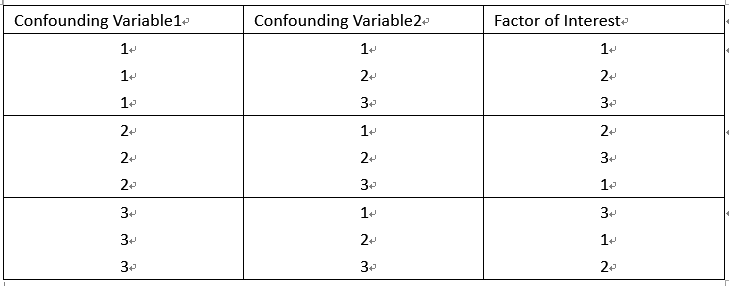
\includegraphics[width=15cm]{cf.png}
        \caption{Latin Square}
        \label{fig:my_label}
    \end{figure}
\vspace{3ex}
\begin{center}
    \Index{Solomon-four Group}
\end{center}
to reduce the effect of pre-post studies on the true measurement after the treatment, we introduce \textbf{Solomon-four Group}.In this method, subjects are randomly assigned to four groups.\\
    Random Select $\rightarrow$ Observe $\rightarrow$ Treat $\rightarrow$ Observe\\Random Select $\rightarrow$ Observe  $\rightarrow$ Observe\\Random Select  $\rightarrow$ Treat $\rightarrow$ Observe\\Random Select  $\rightarrow$ Observe
\vspace{3ex}
\begin{center}
    \Index{Counter Balancing}
\end{center}
It can average the effect of subjects' difference, by giving each subject all the levels of treatment. Each subject is treated with all treatments.

\vfill
\newpage


                                                                                                                                                                                                                                                                                                                                                                                                                                                                                                                                                                                                                                                                                                  

\section{Descriptive Methods of Data}
After doing the research, we have to represent data in a clear and efficient way. In order to do that, we have \textbf{Descriptive Methods of Data}.\\\Index{Raw Data}: Lots of useless number that need to be sorted.\\

\begin{objectives}
    \item Learn how to describe data with numbers
    \item Know different types of graphs
    \item Know advantages and drawbacks of graphs
    \item Know different experiment error and how they are created
\end{objectives}
\subsection{Graphical Descriptive Methods}
\begin{description}
    
    \item[Graphical]:To describe data with Graphs, it is clearer and easier to attain 
    \begin{description}
        \item[Bar Chart]:It is used to compare value easily and clearly. It can have \textbf{Cluster} where high bars gather and \textbf{Gap} where low bars gather.
        \begin{figure}[H]
            \centering
            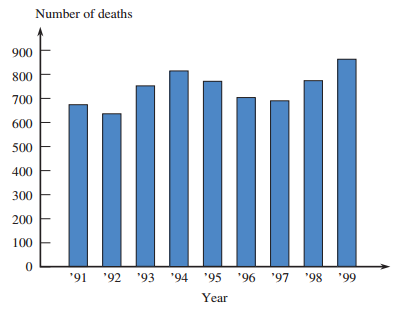
\includegraphics[width=75mm]{bar_chart.png}
            \caption{Bar Chart}
            \label{bar chart}
        \end{figure}
        \item[Dot Plot]: It is used to see which values have the most frequency or the most frequent value of results as well as the distribution of data.
        \begin{figure}[H]
            \centering
            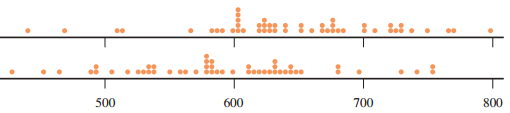
\includegraphics[width=75mm]{dotplot.png}
            \caption{Dot Plot}
            \label{dot plot}
        \end{figure}
        \item[Pie Chart]: It is used to see \textbf{Relative Frequency} or the proportion of different parts.
        \begin{figure}[H]
            \centering
            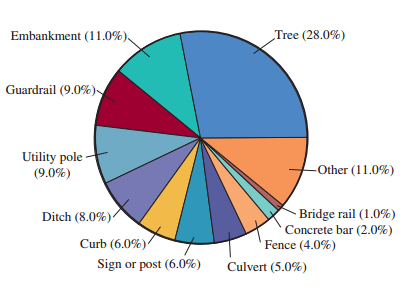
\includegraphics[width=75mm]{pie_chart.png}
            \caption{Pie Chart}
            \label{pie chart}
        \end{figure}
        \item[Segmented Bar Chart]: The same as \textbf{Pie Chart}, just in the form of a bar.
        \begin{figure}[H]
            \centering
            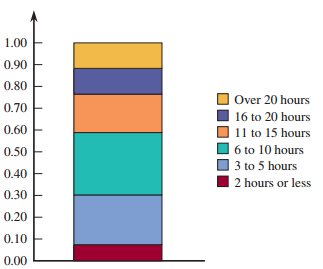
\includegraphics[width=75mm]{segmented_bar_chart.png}
            \caption{Segmented Bar Chart}
            \label{segmented bar chart}
        \end{figure}
        \item[Ogive]: It is used to show the \textbf{Cumulative Frequency}.
        \begin{figure}[H]
            \centering
            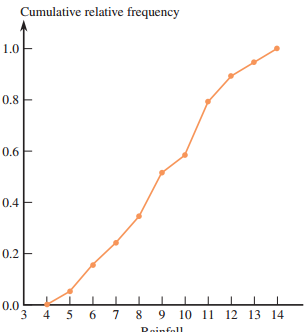
\includegraphics[width=75mm]{crf.png}
            \caption{Ogive}
            \label{crf}
        \end{figure}
        \item[Parete Chart]: The Ogive on the top of the Bar Chart.
        
        \item[Stem and Leave]: It is like a kind of \textbf{Side-way Dot-plot}, can be used to see the distribution of results.
        \begin{figure}[H]
            \centering
            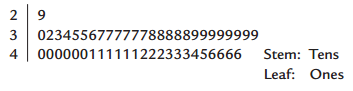
\includegraphics[width=75mm]{stem_leaf.png}
            \caption{Stem and Leaf}
            \label{fig:my_label}
        \end{figure}
        \item[Histogram]: It can be used to show the distribution of data on different \textbf{Class Intervals} which can be \textbf{Continuous or Discrete}.
        \begin{figure}[H]
            \centering
            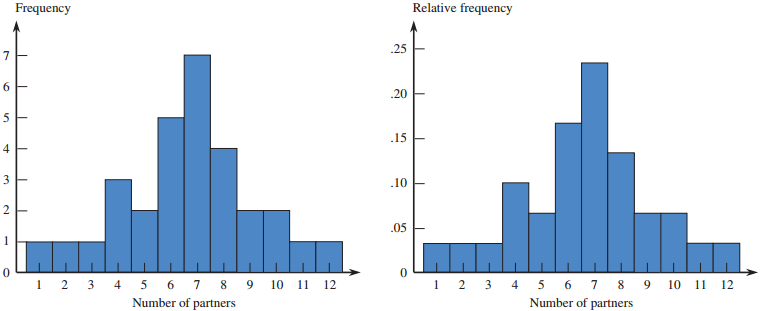
\includegraphics[width=75mm]{histogram.png}
            \caption{Histogram}
            \label{histogram}
        \end{figure}
        \begin{figure}[H]
            \centering
            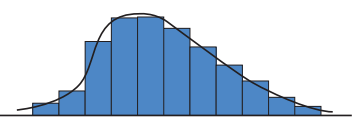
\includegraphics[width=75mm]{smoothed_histogram.png}
            \caption{Smoothed Histogram}
            \label{smoothed histogram}
        \end{figure}
        \item[Box and Whiskers Plot]: It can show the distribution by Right or Left the tail's skewed to.
        \begin{figure}[H]
            \centering
            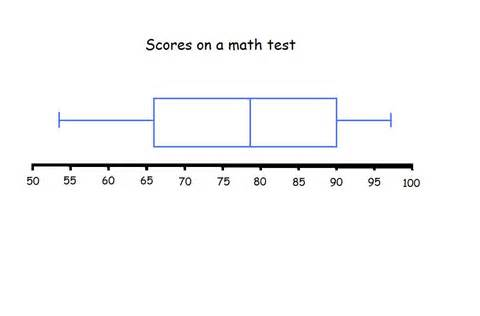
\includegraphics[width=75mm]{th.jpg}
            \caption{Box and Whiskers}
            \label{box and whiskers}
        \end{figure}
        \begin{Question}
            How can Box and Whiskers plot be drawn to a Smooth Histogram
            \solution The narrower the 25 percent, the higher the curve
        \end{Question}
        \item[Scatter Plot]: It can be used to show \textbf{Trends} or \textbf{Correlation} of two factors.
        \begin{figure}[H]
            \centering
            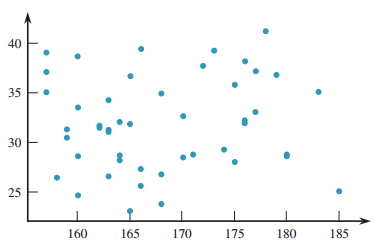
\includegraphics[width=75mm]{scatter.png}
            \caption{Scatter Plot}
            \label{scatter plot}
        \end{figure}
       
        \item[Comparative Bar Chart]: If there are Multiple Samples of \textbf{Categorical Data}.
        \begin{figure}[H]
            \centering
            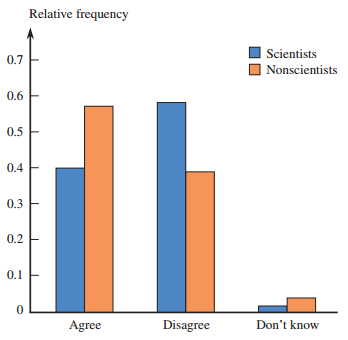
\includegraphics[width=75mm]{comparative_bar_chart.png}
            \caption{Comparative Bar Chart}
            \label{comparative bar chart}
        \end{figure}
    \end{description}
\end{description} 

\subsection{Numerical Descriptive Methods}
Besides using Graphs to represent data, it's also important to know how to describe a data list with numerical descriptive methods to show the features of data clearly and directly.
\begin{itemize}
\item \Index{Describing the Center} When describing numerical data, it is common to report a value that is representative
of the observations. Such a number describes roughly where the data are located or “centered” along the number line, and is called a measure of center. The two most widely used measures of center are the \Index{Mean} and the \Index{Median}.
\begin{itemize}
    \item \textbf{Mean}: The mean of a numerical data set is just the familiar arithmetic average: the sum of the observations divided by the number of observations.
    \begin{equation}
        \bar x=\frac{\Sigma x}{n}
    \end{equation}
    \item \textbf{Median}: Once the data values have been listed in order from smallest to largest, the median is the middle value in the list, and
it divides the list into two equal parts. 
    \item \Index{Mode}: Mode sometimes is used. It is the value that appears in the data set the most often.
\end{itemize}

\item \Index{Describe the Variability}It is also
important to describe how much the observations differ from one another. 
\begin{itemize}
    \item \Index{Range}: The simplest numerical measure of variability is the range. range is the difference between the largest observation and the smallest observation.
    \item\Index{Variance and Standard Deviation}: The customary way to prevent negative and positive deviations from counteracting one another is to square them before combining.
    \begin{equation}
        s_x = \sqrt {\frac{1}{N}\sum\limits_{i = 1}^N {\left( {x_i - \bar x} \right)^2 } }
    \end{equation}
    Variance is just without the square root.
    \item\Index{Interquartile range}: IQR, The difference between the lower quartile and the upper quartile.
    \item \Index{Percentile}: is the median of half of the data set. \Index{Lower quartile Q1}is the median of the lower half, and the \Index{Upper quartile Q3} is the median of the upper half.
\end{itemize}
\end{itemize}
\begin{Question}:
    Do these values count the out-liners?
\end{Question}
\vfill
\newpage





\section{Inferential Methods}

\subsection{Estimation}
\begin{objectives}
    \item Understand the variability of a sample data
    \item Understand Confidence Level
    \item Know how to estimate Population mean with confidence level
\end{objectives}

\subsubsection{Variability of a Sample}
The values in a sample data vary slightly, the population's value even change more.The \Index{sampling variability} of a statistic refers to how much the statistic varies from sample to sample and is usually measured by its standard error
\begin{description}
    \item[Standard Error]a measure of the accuracy of predictions
    \begin{equation}
\sigma =\sqrt[2]{\frac{\Sigma (x\minus \bar x)^{2}}{n}}.
\end{equation}
    \item[Standard Deviation for sample]
    \begin{equation}
    \sigma_{\bar x} = \frac{\sigma}{\sqrt{n}} 
\end{equation}
    \item[Z score] is one type of measure of relative standing. It shows that how many standard deviation away from the mean a value is.
    \begin{equation}
      z=\frac{\bar x-\mu}{\sigma}
    \end{equation}
    \begin{examplebox}{Z score}
      If the population has a mean of 1.0 and a standard deviation of 0.2. Then a data with Z as 1 would has the value of 1.2 which is 1 standard deviation away from the population mean.
    \end{examplebox}
    \item[\Index{Central Limit Theorem}]:  When n is large and the sample size is less than 10 percent of the population size, the statistic
has a sampling distribution that is approximately
normal with mean.
    \item[\Index{Normal Distribution}]: Normal distributions are continuous probability distributions that are bellshaped and symmetric. There are many normal distributions, the \Index{Standard Normal Distribution} has Mean of 0, Standard Deviation of 1.
    \begin{figure}[H]
      \centering
    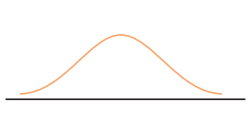
\includegraphics[width=75mm]{normald.png}
    \caption{A Normal distribution}
    \label{Figure}
\end{figure}
    \item[Empirical Rule]:The shape of a normal sampling distribution is defined by \Index{the empirical rule}. The is the statistical rule stating that for a normal distribution, then
Approximately 68\% of the observations are within 1 standard deviation of the
mean.
Approximately 95\% of the observations are within 2 standard deviations of the
mean.
Approximately 99.7\% of the observations are within 3 standard deviations of
the mean.
\begin{figure}[H]
      \centering
    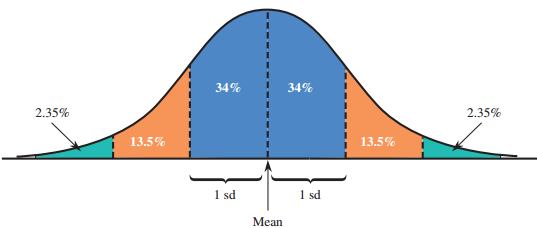
\includegraphics[width=95mm]{er.png}
    \caption{Empirical Rule}
    \label{Figure}
\end{figure}
\end{description}
\begin{Question}
    What if we want to know other percentage of observations correlated to other standard deviation? 
    \solution Use the Calculator.
\end{Question}

\subsubsection{Estimation of Confidence Interval}


\begin{description}
    \item \Index{Confidence Interval}: a confidence interval (CI) is a type of interval estimate of a population parameter.
    \item \Index{Confidence Level}: Confidence level is how frequently the observed interval contains the true parameter if the experiment is repeated, basically how "confident" we are about this estimation.
\\
\begin{examplebox}{Confidence Interval}
    If there is a sample data, we estimate its Confidence Interval for population's mean is 99 to 101 with a Confidence Level of 99\%, then it means we are 99\% sure the true mean of the population is within this range.
\end{examplebox}
\end{description}
 
\paragraph{How to calculate Confidence Interval} To calculate a confidence interval of a certain sample, we use an equation. However the equation varies when the standard deviation \(\sigma\) of the population is know or unknown.
\begin{description}
    \item \textbf{\(\sigma\) is known}:
    We use Z score to estimate.
    \begin{equation}
    \mu=\bar x \pm Z_{c} (\frac{\sigma}{\sqrt{n}} )
    \end{equation}
    \item \textbf{\(\sigma\) is unknown or n<30}:
    We use \Index{t distribution} which is more biased and vary more than normal distribution because the sample size is too small.
    \begin{equation}
    \mu=\bar x \pm t_{c} (\frac{\sigma}{\sqrt{n}} )
    \end{equation}
\end{description}

 \Index{Marginal Error}:It is the deviation the mean can have within a range.
 \begin{equation}
   M.E.= Z_{c} (\frac{\sigma}{\sqrt{n}} )
\end{equation}
\paragraph{How to get \(z_c\) or \(t_c\)}In order to get \(z_c\) and \(t_c\), we use the given confidence level. 
\begin{figure}[H]
      \centering
    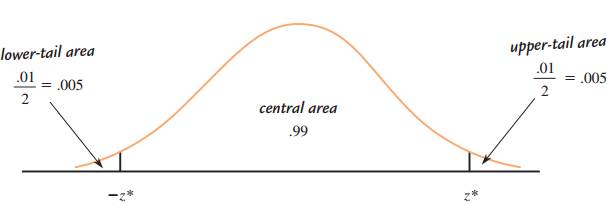
\includegraphics[width=95mm]{meanestimate.png}
    \caption{Confidence Interval}
    \label{Figure}
\end{figure}
\begin{examplebox}{Get \(z_c\)}
    If the confidence level is 90\%, then it means the confidence level should cover 90\% of the area in a sample's distribution curve, then we use this information to type in calculator to get it.
\end{examplebox}

\begin{Question}
    How about t distribution
    \solution Use the t-dis button on the calculator and do the same thing
\end{Question}

\subsection{Hypothesis Test}
\begin{objectives}
    \item Know Null hypothesis
    \item Distinguish \(H_a\) and \(H_0\) hypothesis
    \item Know how to test hypothesis with \(z_c\) and z
    \item Know p-value as significance level
\end{objectives}
\vbox{}
We have use a sample and its values to infer its population's mean.

\subsubsection{Hypothesis}
\Index{Hypothesis}: A hypothesis is a claim or statement about the value of a single population characteristic or the values of several population characteristics. 
\begin{itemize}
    \item \Index{Null Hypothesis}: The null hypothesis, denoted by \(H_0\), is a claim about a population characteristic that is initially assumed to be true.
    \item \Index{Alternative Hypothesis}: denoted by \(H_a\), is the competing claim.
\end{itemize}
\begin{examplebox}{Hypothesis}
    \(H_a\): \(\mu <3\) \\
    \(H_0\): \(\mu =3\)
\end{examplebox}

\subsubsection{Errors in Hypothesis Testing}
In this section, we discuss
the kinds of errors that can occur and consider how the choice of a test procedure
influences the chances of these errors.
\begin{description}
    \item[\Index{Type I Error}]: the error of rejecting \(H_0\) when \(H_0\) is true.The \textbf{\Index{probability of a type I error occurs}} is denoted by \(\alpha\)
    \begin{center}
        \(\alpha\)=P( reject \(H_{0}\) | \(H_{0}\) is true)
    \end{center}
    \item[\Index{Type II Error}]:the error of failing to reject \(H_0\) when \(H_0\) is false.The \textbf{\Index{probability of a Type II error}} is denoted by \(\beta\).
    \begin{center}
        \(\beta\)=P( fail to reject \(H_{0}\) | \(H_{0}\) is false)
    \end{center}
\end{description}
\begin{examplebox}{Error}
    A researcher wants to compare the speed  of two cars. The null and alternative hypotheses are:
\begin{itemize}
    \item Null hypothesis (\(H_{0}\)): \(\mu_{1}=\mu_{2}\); The two cars are the same fast
\item Alternative hypothesis (\(H_{a}\)): \(\mu_{1}\neq \mu_{2}\); The two cars are not the same fast.
\end{itemize}
A type I error occurs if the researcher rejects the null hypothesis and concludes that the two cars are different but in fact they are not.  \\
A type II error occurs if the researcher fails to reject the null hypothesis when it should be rejected. That is, the researcher concludes that the cars are the same when, in fact, they are different. 
\end{examplebox}

\subsubsection{Testing Hypothesis}
Now that the basic concepts of hypothesis testing have been introduced, we are ready
to turn our attention to the development of procedures for using sample information
to decide between a null and an alternative hypothesis. There are two possible conclusions: We either reject \(H_0\) or we fail to reject \(H_0\).
\\
\begin{description}
    \item[\Index{P-Value or Observed Significance Level}]: A measure of inconsistency between the hypothesized value for a population characteristic and the observed sample. It is the probability, assuming that \(H_0\) is true,
of obtaining a test statistic value at least as inconsistent with \(H_0\) as what was
observed.
    \item[\Index{Significance Level}]: The significance level is the highest value of a probability value for which the null hypothesis is rejected.
    \item[\Index{Test Statistic}]: A test statistic is computed using sample data and is the value used to reach a
conclusion to reject or fail to reject \(H_0\).
\end{description}

\paragraph{How to test}: Depending on the \(H_a\), we have \Index{One tail test} and \Index{Two tail test}

\begin{figure}[H]
    \centering
    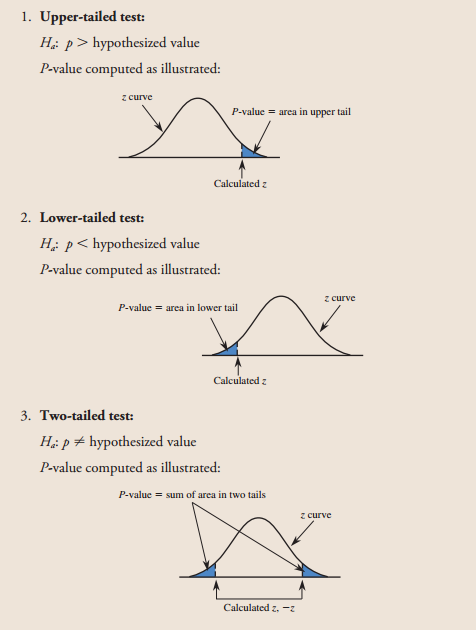
\includegraphics[width=125mm]{testhp.png}
    \caption{One-tail Test and Two-tail Test}
    \label{Figure 2}
\end{figure}

\textbf{Steps on Testing}
\begin{enumerate}
    \item Describe the population characteristic about which hypotheses are to be tested
    \item State the null hypothesis \(H_0\).State the alternative hypothesis \(H_a\).
    \item Select the significance level a for the test.
    \item Display the test statistic to be used, with substitution of the hypothesized
value identified in Step 2 but without any computation at this point.
    \item Check to make sure that any assumptions required for the test are reasonable.
    \item Compute all quantities appearing in the test statistic and then the value of
the test statistic itself.
    \item Determine the P-value associated with the observed value of the test statistic.
    \item State the conclusion 
    \begin{itemize}
    \item \textbf{If p-value<\(\alpha\), then we reject \(H_0\)}
    \item \textbf{If p-value>\(\alpha\), then we fail to reject \(H_0\)}
\end{itemize}
\end{enumerate}

\begin{Question}
    Are \(\alpha\) and Confidence Level connected?
    \solution The confidence interval at confidence level \(1-\alpha\%\) for a population statistic contains \(1-\alpha\%\) of data. So for example, the significance level is 5\% if the confidence level is 95\%
\end{Question}
\subsubsection{Power}
\Index{Power of a Test}: The power of a test is the probability of rejecting the null hypothesis
\begin{equation}
    Power=1-\beta
\end{equation}
\begin{center}
    \(1-\beta\)=P( reject \(H_{0}\) | \(H_{0}\) is false)
\end{center}
\begin{figure}[H]
    \centering
    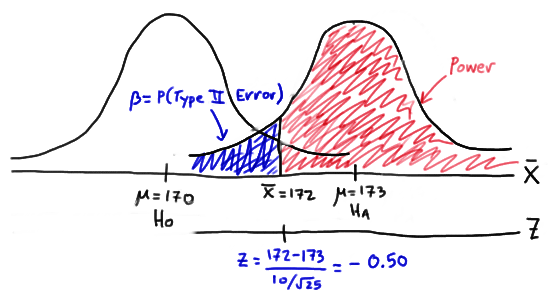
\includegraphics[width=110mm]{power.png}
    \caption{Power}
    \label{Figure}
\end{figure}
\begin{Question}
    How do get p-value?
    \solution we use the corresponding Z to type into calculator to get the area of the uncovered area.
\end{Question}

\subsection{Sample Size}
\begin{objectives}
    \item Understand the effect of sample size on sample
    \item Know how to calculate the smallest sample size to get a certain Margin Error
\end{objectives}
\vbox{}
The sample size n is very important to a sample data's distribution, the bigger n becomes, the more normal the distribution become and the closer the data is to the true population mean.\\
\vbox{}
So,the bigger the sample size, the smaller the Margin error becomes.\\
\vbox{}
From the previous chapter, we know the equation of Marginal Error is
\begin{equation}
   M.E.= Z_{c} (\frac{\sigma}{\sqrt{n}} )
\end{equation}
If we change the equation and solve for n, we get the following equation for n
\begin{equation}
    n=\frac{z^{2}\times \sigma^{2}}{(M.E.)^{2}}
\end{equation}
\begin{examplebox}{Minimum Sample Size}
    Q: We want to estimate the average age of the workers, to \(\pm 1 year\), with a confidence level of 95\%. The standard deviation of the poupulation is 0.1.How big should the sample be? \\
According to the question, we can know the given value, M.E.=\(1 year\) and C.L.=\(0.95\). \\
Use the C.L. to get the Z value with calculator.\\
Plug these number in the equation \(n=\frac{z^{2}\times \sigma^{2}}{(M.E.)^{2}}\)\\
Then roung n to the nearest integer.
 
\end{examplebox}

\chapter{Univariate Data}

\vfill
\pagebreak

\section{Comparing Populations}

\subsection{Differences between Means}

\subsubsection{Sampling Distribution of Differences between Means}
\begin{objectives}
    \item Compute mean, standard error, variance of differences of means
    \item Compute the probability of a difference between means being above a specified
    value
    \item Calculate a Confidence Interval of difference between means with a specific confidence level
       \item Test the differences of two means
    \item Calculate t and p for difference of means
\end{objectives}
\vbox{}
For statistical analyses, it is often more important to concern for difference between means. For example, the difference of means of a control group and an experiment group.
The \Index{Sampling Distribution of Difference between Means} can be though of select samples from each population and get their differences of means repeatedly.
\vbox{}
\\Then, naturally we can know \Index{mean of the sampling distribution of the difference
between means} the mean of the distribution of differences between sample means
is equal to the difference between population means
\begin{equation}
    \mu_{M1-M2}=\mu_1-\mu_2
\end{equation}
As for \Index{variance of the sampling distribution of the difference between
means}
\begin{equation}
    {\sigma^{2}}_{M1-M2}={\sigma^{2}}_{M1}+{\sigma^{2}}_{M2}
\end{equation}
the variance of the sampling distribution of the difference between
means is equal to the variance of the sampling distribution of the mean for
Population 1 plus the variance of the sampling distribution of the mean for
Population 2.
\\We can replace the sample's variance with population's variance:
\begin{equation}
    {\sigma^{2}}_M=\frac{\sigma^{2}}{N}
\end{equation}
If the Variance and Sample Sizes are the same, we can simplify the equation to be:
\begin{equation}
    {\sigma^{2}}_{M1-M2}=\sqrt{\frac{2\sigma^2}{n}}
\end{equation}

\paragraph{\textbf{How to calculate the probability of difference of means being above of below a value}}
:This is the same as to calculate the proportion of a normal distribution being above or below a value. We just use the calculator and type in the standard deviation and mean of this distribution and find the proportion.
\begin{figure}[H]
        \centering
            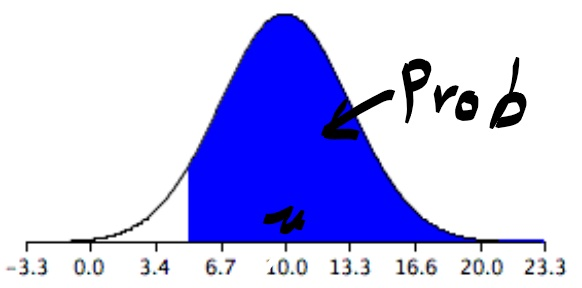
\includegraphics[width=80mm]{prob1.jpg}
            \caption{Probability for being above}
            \label{Probability for being above}
\end{figure}

\textbf{Estimate Confidence Interval}
\\The process is basically the same as calculating the confidence interval for mean of one population. We just have replace several terms.
\\There are three important assumptions for estimating Confidence Interval:
\begin{enumerate}
    \item Variances of the two populations are the same. It's also know as \Index{assumption of homogeneity of variance}.
    \item Difference of means has \textbf{Normal Distribution}.
    \item Every value is independently sampled.
\end{enumerate}
The equation for \Index{Confidence Interval of Difference between Means}:
\begin{equation}
    (M1-M2)\pm (t_{c.l.})(S_{M1-M2})
\end{equation}
\(t_{c.l.}\) should be computed with the calculator using specific \textbf{degrees of freedom}:
\begin{equation}
    d.f.=(n_1-1)+(n_2-1)
\end{equation}
where n is the sample size of two populations
\\ \(S_{M1-M2}\) should be computed with given variance:
\begin{equation}
    S_{M1-M2}=\sqrt{\frac{{\sigma_1}^2+{\sigma_2}^2}{n}}
\end{equation}

\Index{MSE}: The estimate of \(\sigma^2\) which is the assumed same variance of two populations.
\begin{equation}
    MSE=\frac{{\sigma_1}^2+{\sigma_2}^2}{2}
\end{equation}
\Index{SSE}: Sum of squared error. Sometimes the sample sizes of two means are different, and we need SSE:
\begin{equation}
    SSE= \sum\left (x-M1 \right )^{2}+\sum \left ( x-M2 \right )^{2}
\end{equation}

\textbf{Hypothesis Test}
The means of two populations sometimes do not matter, what is important is that if there is actually a difference between the means of populations. 
\\
\begin{examplebox}{Difference between Means}
    If there is a new drug, researchers have to compare the mean of the control group and experiment group. Only the difference actually matters, it's important to know if it exists and how big it is.
\end{examplebox}
\vbox{}
There are three important assumptions for testing if the Difference exists:
\begin{enumerate}
    \item Variances of the two populations are the same. It's also know as \Index{assumption of homogeneity of variance}.
    \item Difference of means has \textbf{Normal Distribution}.
    \item Every value is independently sampled.
\end{enumerate}

The test is just like estimating the probability of rejecting the null hypothesis we learnt before:
\begin{equation}
    t=\frac{(M1-M2)-0}{S_{M1-M2}}
\end{equation}
\(M1=M2\) is the tested statistic, 0 is the hypothesized value(Null Hypothesis)

\textbf{P-value} is just the probability of being greater than the absolute value of t, we compute it using a calculator like before with specific degrees of freedom like we introduced before.
\\After we compute the P-value, we can conclude:
\begin{itemize}
   \item \textbf{If p-value<\(\alpha\), then we reject \(H_0\)}
    \item \textbf{If p-value>\(\alpha\), then we fail to reject \(H_0\)}
\end{itemize}
\begin{Question}
    What is Pooled variance? When do we use it?
\end{Question}

\subsection{All Pairwise Comparisons among Means}
We have to compare more than two means and compare each pair of means. Then as more means being compared, the probability of Type One Error increases. So to eliminate this problem, we introduce the \Index{Tukey HSD test} with \Index{studentized range distribution}.
\begin{examplebox}{All Pairwise Comparison}
    We want to know weather's effect on people's math performance. Then we have to compare sunny, rainy, snowy, windy, and foggy with each other.
\end{examplebox}

\vbox{}
\textbf{Steps of Tukey HSD Test}
\begin{enumerate}
    \item Compute the Variance and Mean for each group
    \item Compute MSE, the mean of variace
    \item Compute Q: 
    \begin{equation}
        Q=\frac{M_i-M_j}{\sqrt{MSE}}
    \end{equation}
    \item Compute P using a specific calculator
\end{enumerate}

\begin{figure}[H]
        \centering
            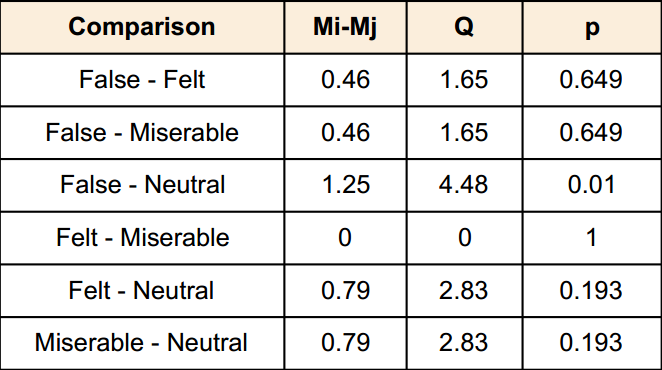
\includegraphics[width=80mm]{Tukey.png}
            \caption{Tukey HSD Test}
            \label{Tukey HSD Test}
\end{figure}
\begin{examplebox}{Tueky Test conclusion}
    For the test result above, what can we conclude?
    \\The false smile is higher than the control
and that the miserable smile is either (a) equal to the false smile, (b) equal to the
control, or (c) somewhere in-between
\end{examplebox}
\subsection{Specific Comparison}
\begin{objectives}
    \item Know Linear Combination
    \item Express Linear Combination with coefficients and means
    \item Do significance test for specific comparison
    \item Know error rates 
\end{objectives}
\vbox{}

Sometimes we have to a more complex comparison between means for more variables, how do we test Significance for the difference?
\\
\begin{examplebox}{More complex comparison}
    We have the scores for students that can be classified as male or female; tall or short. The scores can be compared between the groups with the free combination of gender and length. Through the test, we wish to know which comparison actually make a difference.
\end{examplebox}
\vbox{}
 \textbf{Steps of Test:}
\begin{enumerate}
    \item Express this difference in terms of a linear combination
using a set of coefficients and the means
    \item Compute L-\Index{Linear Combination}: The computation each means times one over total result and add together, same value we got when we computed the difference between means
    \begin{equation}
        L=\sum c_iM_i
    \end{equation}
    where \(c_i\) is the ith coefficient and \(M_i\) is the ith mean
    \item Compute t for testing L for Significance
    \begin{equation}
        t=\frac{L}{\sqrt{\frac{\sum {c_i}^2 MSE}{n}}}
    \end{equation}
    \item Use the calculator to find two-tailed probability and conclude
\end{enumerate}
\begin{Question}
    How do we use L to get p-value? What do we compare p to?
\end{Question}
\vbox{}
\textbf{Multiple comparison}
\\As we add more and more comparison, it's more possible to make Type one error, we need to distinguish two error rates:
\begin{itemize}
   \item \Index{per-comparison error rate}: the probability of a Type I error for a particular comparison.
   \item \Index{familywise error rate(FW)}: the probability of making one or more Type I errors in a family or set of comparisons.
\end{itemize}

\subsection{Correlated Pairs}
\begin{objectives}
    \item Tell if you have Correlated Pairs instead of Independent Group
    \item Do significance test for Correlated Pairs    
\end{objectives}
\vbox{}
Sometimes when we compare means, we cannot compare them with the test we introduce before, because they are not independent. They are related to each other. So they are \Index{Correlated Pairs}, what we discuss before are \Index{Independent Pairs}.
\\
\begin{examplebox}{Correlated Pairs}
     If the experiment is test the effect of a new drug on the disease. The subjects take the new drug or placebo and are measured. There is only one group of subjects,
each subject being tested in both the conditions. The means are correlated.
\end{examplebox}
\vbox{}
\textbf{Steps for test of Correlated Pairs}
\begin{enumerate}
    \item Compute the difference of scores of each subject
    \item Do the test of a single mean for the mean of differences between means.
\end{enumerate}
correlated t tests  have more power than
independent-groups t tests, because standard error of the difference between means is smaller in the correlated t
test and, since this term is in the denominator of the formula for t, results in a
larger t.


\section{Analysis of Categorical Data}

\subsection{Graphical Descriptive Methods}
\begin{objectives}
\item Briefly review the graphs for presenting categorical data
\item Know the advantages of various graphs
\end{objectives}
\vbox{}
After doing the research and getting a bunch of categorical Raw Data, it's important for us to sort and represent this data in a clear and efficient way so that we can do the following analysis of data.\\
\begin{Center}
    \Index{Comparative Bar Chart}
\end{Center}
This kind of bar charts can give a straightforward comparison between different groups in terms of the \textbf{Relative Frequency}. But remember when comparing, we compare the \textbf{Relative Frequency} instead of frequency.
\begin{figure}[H]
            \centering
            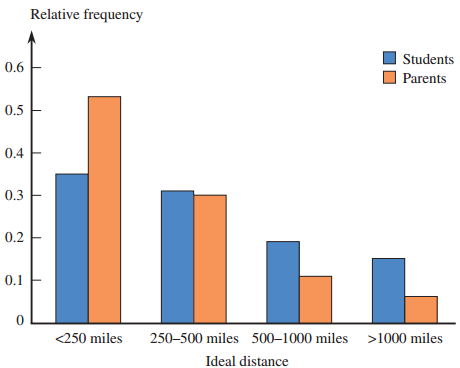
\includegraphics[width=75mm]{cbc.png}
            \caption{Comparative Bar Chart}
            \label{Comparative Bar Chart}
        \end{figure}
\begin{Center}
    \Index{Pie Chart}
\end{Center}
The proportion of each category is representing by the size of its correlated segment's area. So it is straightforward to see the \textbf{Relative Frequency} of each category.
        \begin{figure}[H]
            \centering
            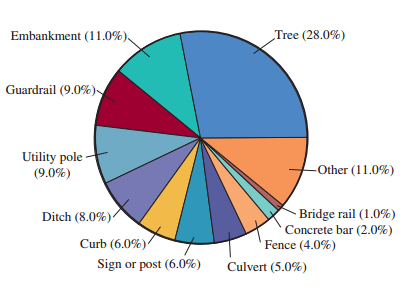
\includegraphics[width=75mm]{pie_chart.png}
            \caption{Pie Chart}
            \label{pie chart}
        \end{figure}
\begin{Center}
    \Index{Segmented Bar Chart}
\end{Center}
It is almost the same as Pie Chart. Instead of a circle , the Segmented Bar chart is a rectangular. It is also straightforward to see the \textbf{Relative Frequency} of each category.
    \begin{figure}[H]
            \centering
            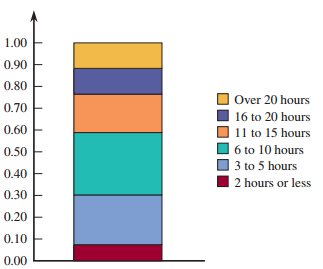
\includegraphics[width=75mm]{segmented_bar_chart.png}
            \caption{Segmented Bar Chart}
            \label{segmented bar chart}
        \end{figure}

\subsection{Numerical Descriptive Methods}
\begin{objectives}
    \item Understand Frequency, Relative Frequency and Proportion of Success
    \item Know how to calculate Relative Frequency and Proportion of Success
\end{objectives}
\vbox{}
Besides representing data by using graphs, there are also two most important features of each category in a research: \textcolor{red}{Frequency} and \textcolor{red}{Relative Frequency}, also there is a special type of Relative Frequency is called \textcolor{red}{Proportion of Success}.\\
\begin{description}
    \item \Index{Frequency}: Frequency is the number of times the category appears in the data set. 
    \item \Index{Relative Frequency}:Relative frequency is the proportion of a certain category within all data.
    \begin{examplebox}{Frequency and Relative Frequency}
    We conduct an interview about BNDS students' favorite color. And there are 500 results in total. Among all these results, the color "red" appears for 50 times, so its frequency is 50, relative frequency is 50/500=0.1.
    \end{examplebox}
    \item \Index{Proportion of Success}: A special relative frequency, when the data has only two categories, we can define one as success and the other one as failure.\\
    \begin{examplebox}{Proportion of Success}
        We are testing BNDS students' AP statistics scores. A 5 is success, a below 5 is failure. And among 100 students, 95 get a 5. So the proportion of success is 95/100=0.95.
    \end{examplebox}
\end{description}

\subsection{Proportion of Success}
\begin{objectives}
    \item Understand dychotomy and proportion of success
    \item Know how do infer Confidence Level of \(\Pi\)
    \item Know how to do hypothesis test of \(\Pi\)
    \item Understand difference of proportion of success
    \item Know how to do confidence interval and hypothesis test for difference of proportion of success
\end{objectives}
\vbox{}
For categorical data, there is a very special case, which has only two categories.\\

\begin{description}
    \item \Index{Dychotomy} : When there are only two possible cases in uni variate data, and we can assign each case as either \textcolor{blue}{success} and \textcolor{blue}{failures}.
    \item \Index{Binomial Distribution} : Used to analyze Dychotomy and as long as n is greater than 30, and the skewness is not too extreme  the Binomial Distribution can be approximate by a \textcolor{red}{Normal Distribution} with the same Mean and Standard Deviation.
    \item \Index{Proportion of Success} : In the Binomial Distribution
    \begin{equation}
        \Pi=\frac{x}{n}
    \end{equation}
    \textbf{x} is number of success in \textbf{n} trials.
    \item \Index{Probability of Success on a trial} : it's denoted by \textbf{p}, it's the same as \(\Pi\). Also, the \(1-p\) is \textbf{q}.
        \begin{equation}
        p=\frac{x}{n}
    \end{equation}
\end{description}

Through a series of deduction, we attain the following equations for the \Index{Expected value of x} and \Index{Variance of x}.
\begin{equation}
    E(x)=np
\end{equation}
\begin{equation}
    Var(x)=np(1-p)
\end{equation}

If we have a sampling distribution for \(Pi\), the \textcolor{blue}{mean} and \textcolor{blue}{standard deviation} are as following:
\begin{equation}
    E(\Pi)=p    
\end{equation}
\begin{equation}
    Var(\Pi)=\frac{p(1-p)}{n}
\end{equation}

\vspace{5ex}
\begin{Center}
    \textbf{Confidence Interval of Proportion of Success}
\end{Center}
Using the equations above of mean and standard deviation, based on our study for Confidence Interval, we can attain the equation for \textcolor{red}{Confidence Interval of Proportion of Success}
\begin{equation}
    \Pi\in(\hat{p}\pm B_{C.L.}\sqrt{\frac{p(1-p)}{n}})
\end{equation}
As mentioned before: as long as n is greater than 30, and the skewness is not too extreme  the Binomial Distribution can be approximate by a \textcolor{red}{Normal Distribution} with the same Mean and Standard Deviation. \textcolor{blue}{\(B_{C.L.}\)} can be approximated by \textcolor{blue}{\(Z_{C.L.}\)}.\\
As for \textcolor{red}{\(\hat{p}\)}, it is the \textcolor{blue}{expected value of p}, which can be calculated by doing \(\frac{x}{n}\) of the sample.

\vspace{5ex}
\begin{Center}
    \textbf{Hypothesis Test of Proportion of Success}
\end{Center}
Based on the equations above and the test value we learnt before, we can attain the equation for the \textcolor{red}{Test Value}.
\begin{equation}
    Z_{T}=\frac{\hat{p}-\Pi_{0}}{\sqrt{\frac{\hat{p}(1-\hat{p})}{n}}}
\end{equation}
As for the test part, it's the same as before.

\vspace{5ex}
\begin{Center}
    \textbf{Sample Size of Proportion of Success}
\end{Center}
When we wish to design a dycholomous experiment, with certain \textcolor{blue}{Confidence Level} and \textcolor{blue}{Margin of Error}. The minimum required \textcolor{red}{Sample Size}:
\begin{equation}
    n=(\frac{Z}{M.E.})^2p(1-p)
\end{equation}
Without the information about the value of p, we take the max value of \(p(1-p)\) which is \(\frac{1}{4}\). Then the equation becomes:
\begin{equation}
    n=(\frac{Z}{2M.E.})^2
\end{equation}

\vspace{5ex}
\begin{paragraph}{Difference of Proportion of Success}
    When we are analyzing, sometimes we care more for the Difference of Proportion of Success between two population, first we discuss for \textcolor{red}{Independent Samples} . \\
    \begin{examplebox}{Difference of Proportion of Success}
           We want to know if the effect of drug changes the percentage of students with 5 on AP test, we concern more for if there is actually a difference for their proportion of success instead of the value of it.
    \end{examplebox}
 \end{paragraph}
 \vspace{6ex}
 \begin{Center}
     \textbf{Confidence Interval for Difference of Proportion of Success}
 \end{Center}
 For the confidence interval of difference of proportion of success, it's technically the same as for difference of mean. We change the expected value to the difference of proportion of success, and the standard deviation to the sum of two standard deviation.
 \begin{equation}
     (\Pi_1-\Pi_2)\in((\hat{p}_1-\hat{p}_2)\pm Z_{C.L.}\sqrt{\frac{\hat{p}_1(1-\hat{p}_1)}{n_1}+\frac{\hat{p}_2(1-\hat{p}_2)}{n_2}})
 \end{equation}
\(\hat{p}\) is just calculated from the sample's x and n, \(Z_{C.L.}\) approximates \(B_{C.L.}\).
\vspace{5ex}
\begin{Center}
    \textbf{Hypothesis Test for Difference of Proportion of Success}
\end{Center}
For the \textcolor{blue}{independent samples the difference of proportion test} is 
\begin{equation}
    Z_{T}=\frac{(\hat{p}_1-\hat{p}_2)-\Pi_0}{\sqrt{\frac{\hat{p}_1(1-\hat{p}_1)}{n_1}+\frac{\hat{p}_2(1-\hat{p}_2)}{n_2}}}
\end{equation}
Where \(\Pi_0=\Pi_1-\Pi_2\) is the hypothesized difference of proportions. And this only works for large n(more than 30).\\
\vspace{5ex}

If this is \textcolor{red}{dependent samples}, then the variance of the difference of proportions should not simply be the sum of two variances, it is:
\begin{equation}
    Var(\hat{p}_1-\hat{p}_2)=Var(\hat{p}_1)+Var(\hat{p}_2)-2Covar(\hat{p}_1,\hat{p}_2)
\end{equation}
Whern \(Covar(\hat{p}_1,\hat{p}_2)\) is resulted by the relation of two samples, and it is:
\begin{equation}
    Covar(\hat{p}_1,\hat{p}_2)=-\frac{\hat{p}_1\hat{p}_2}{n}
\end{equation}
Here, we are assuming that \textcolor{blue}{sample size of two populations are the same n}. \\
Except for the variation of variance, the other processes are exactly the same with independent samples.

\include{chapter_categorical}

\chapter{Bivariate}

\vfill
\pagebreak

\section{Regression}

\subsection{Bivariate Numerical Data Descriptive Methods}
\begin{objectives}
    \item Know how to draw graph for bivariate data
    \item Understand linear regression
    \item Know how to do regression for bivariate data
\end{objectives}
\vbox{}
\Index{Bivariate Data} is the set of numerical data from two measurements of a sample. These two measurements may have some kind of correlation and we need to represent this correlation using graphical method and linear regression.\\
\begin{examplebox}{Bivariate}
    We want to know the if there is a cause-effect relationship between students' AP stats score and time spent on practice problems, then we measure individual in the sample for score and practice time. The data has two variables in pairs.
\end{examplebox}
\begin{Center}
    \textbf{Graphical method}
\end{Center}
We use \textcolor{red}{Scatter-plot}. y is the \textcolor{blue}{Response Variable}, x is the \textcolor{blue}{Experimental Variable}. We draw them in one graph intending to find the \textcolor{red}{Cause-effect relation} between the two factors. In this scatter-plot, it's acceptable to have two y for the same x.
\begin{figure}[H]
    \centering
        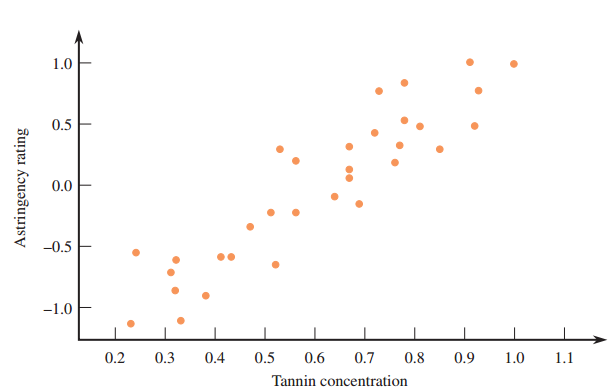
\includegraphics[width=100mm]{relation.png}
        \caption{Scatter-plot}
        \label{fig:my_label}
\end{figure}
From the example of representing bi-variate data using a scatter-plot above, we are able to see the pattern and relationship between x and y very clearly. In this example, it's clear that the response variable is positively related to the explanatory variable x. The relationship is roughly linear.
\vspace{6ex}
\begin{Center}
    \textbf{Regression}
\end{Center}
It's easy to observe that in the above scatter-plot there is a linear relation between x and y. And doing regression is we try to find a \textcolor{red}{linear function that can best represent the cause-and-effect relationship} between two features of one sample. We can do the regression using calculator.

\begin{equation}
    \hat{y}=b_0+b_1x_i
\end{equation}
Where \(\hat{y}\) is the \Index{y predicted}, \(b_0 b_1\) are two constants.\\
\begin{paragraph}{Residual}
    Though we try to find the best, there is difference between the predicted value and the actual value. This difference is called as the \Index{Residual}: The error due to regression, also the unexplained deviation.
\end{paragraph}
\begin{equation}
    e_i=y_i-\hat{y}_i
\end{equation}
The linear function we are looking for is the one that minimizes the \Index{Sum of Square Residuals/SSR}. This method of doing regression is \Index{Least Square Regression}.
\begin{equation}
    \sum{{e_i}^2}=\sum{(y_i-\hat{y}_i)^2}
\end{equation}
\Index{Time Series}: When we have repeated measurements for several times, we can think of it as Bivariate data, where the x-axis is time. The points on the time-series though have to be connected starting from the origin. In a time-series, we can find \textcolor{red}{trend} of the variable we are considering.
\begin{figure}[H]
    \centering
        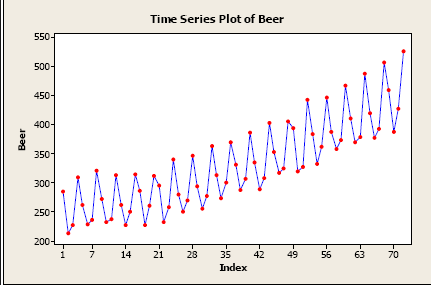
\includegraphics[width=100mm]{times.png}
        \caption{Time series}
        \label{fig:my_label}
\end{figure}

\subsection{More about Regression}
\begin{objectives}
    \item Understand coefficients in a regression
    \item Know variability of a regression    
\end{objectives}
\vbox{}
With a bunch of data of x and y, how do we calculate the two important constants in the linear regression \(\hat{y}=b_0+b_1x_i\)?
 \vspace{6ex}
\begin{Center}
    \textbf{Variance and Covariance}
\end{Center}
    First, we need to calculate the \textcolor{red}{variance} and \textcolor{red}{Covariance} of all x and y data.
    \begin{equation}
        Var(x)=\frac{\sum{(x_i-\bar{x})(x_i-\bar{x})}}{n}    
    \end{equation}
    \begin{equation}
        Var(y)=\frac{\sum{(y_i-\bar{y})(y_i-\bar{y})}}{n}
    \end{equation}
    \begin{equation}
        Covar(x,y)=\frac{\sum{(x_i-\bar{x})(y_i-\bar{y})}}{n}
    \end{equation}
\begin{itemize}
    \item \Index{Variance}: The measure of the average deviation form the mean.
    \item \Index{Covariance}: The measure of how much of the variability in the response variable(y) can be explained by the variability in the explanatory variability(x).
\end{itemize}
And based on the above equations, we can get some other equations.
\begin{equation}
    S_{xx}=\sum{(x_i-\bar{x})^2}=nVar(x)
\end{equation}
\begin{equation}
    S_{yy}=\sum{(y_i-\bar{y})^2}=nVar(y)    
\end{equation}
\begin{equation}
    S_{xy}=\sum{(x_i-\bar{x})(y_i-\bar{y})}=nCovar(x,y)
\end{equation}
 \vspace{6ex}
\begin{Center}
    \textbf{Coefficient}
\end{Center}
Well, using the above equations for variance, through a long way of deduction, we can get the equations of the two constants in the linear regression.
\begin{equation}
    b_1=\frac{Covar(x,y)}{Var(x)}
\end{equation}
\begin{equation}
    b_0=\bar{y}-b_1\bar{x}
\end{equation}
Also, using the equations we can do some deduction.
\begin{align}
    \because  \ b_0=\bar{y}-b_1\bar{x}\\
    \therefore  \ \bar{y}=b_0+b_1\bar{x}\\
    \hat{y}(\bar{x})=\bar{y}
\end{align}
So we know that the \textcolor{red}{line of best fit definitely passes through the point \((\bar{x},\bar{y})\)}.
 \vspace{6ex}
\begin{Center}
    \textbf{Deviation}
\end{Center}
Deviation is difference between each y and mean of all y. And it can be divided into two parts. \textcolor{blue}{Total Deviation=Unexplained Deviation+Explained Deviation}
\begin{equation}
    (y_i-\bar{y})=(y_i-\hat{y}_i)+(\hat{y}_i-\bar{y})
\end{equation}
\begin{align}
    SST=\sum{(y_i-\bar{y})^2}\\
    SSR=\sum{(y_i-\hat{y}_i)^2}\\
    SSE=\sum{(\hat{y}_i-\bar{y})^2}
\end{align}
\begin{align}
    \because \ (y_i-\bar{y})=(y_i-\hat{y}_i)+(\hat{y}_i-\bar{y})\\
    \therefore \ SST=SSR+SSE
\end{align}
We should also know that \textcolor{red}{explained deviation is independent form unexplained deviation}.

\subsection{Evaluation of the Regression}
\begin{objectives}
    \item Understand coefficient of determination
    \item Understand Pearson's coefficient of correlation
    \item Know z-scores to evaluate the relationship
\end{objectives}
\vbox{}
After we collect data of two variables x and y and do the best fit regression, how do we know there is actually a cause-and-effect relationship between x and y and the regression model is good enough?
\vspace{3ex}
\begin{Center}
    \textbf{Z-scores}
\end{Center}
Using Z-score is one way to judge if there is a linear relationship between x and y.
\begin{align}
    Z_{x_i}=\frac{x_i-\bar{x}}{S_x}\\
    if\ x_i>\bar{x}\ then\ Z_{x_i}>0\\
    if\ x_i<\bar{x}\ then\ Z_{x_i}<0
\end{align}
\begin{align}
    Z_{y_i}=\frac{y_i-\bar{y}}{S_x}\\
    if\ y_i>\bar{y}\ then\ Z_{y_i}>0\\
    if\ y_i<\bar{y}\ then\ Z_{y_i}<0
\end{align}
If \textcolor{red}{there is a linear relationship} between x and y, then 1) or 2) below must be true. Meaning:
\begin{enumerate}
    \item \(\sum{Z_{x_i}Z_{y_i}}>>0\)
    \item \(\sum{Z_{x_i}Z_{y_i}}<<0\)
\end{enumerate}
If \textcolor{blue}{there is NO linear relationship} between x and y, when \(Z_{x_i}>0\), sometimes \(Z_{y_i}>0\) and sometimes \(Z_{y_i}<0\). Meaning:
\begin{itemize}
    \item \(\sum{Z_{x_i}Z_{y_i}}\approx 0\)
\end{itemize}
\vspace{3ex}
\begin{Center}
    \textbf{Coefficient of Determination}
\end{Center}
Even though we might get a regression model that seems OK, we still have to question that if we have taken all factors into consideration. So we have the Coefficient of Determination:
\begin{description}
    \item[\Index{Coefficient of Determination}]: Also known as \Index{\(R^2\)}. It tells us the \textcolor{red}{Proportion of the data explained by the model}.
\end{description}
\begin{equation}
    R^2=\frac{SSE}{SST}
\end{equation}
The higher \(R^2\) is, the more the regression model can explain the change in data. So the range of it is:
\begin{equation}
    R^2 \in (0,1)
\end{equation}
\begin{itemize}
    \item The closer \(R^2\) is to 1, the more data in the sample is being explained by the model.
    \item The closer \(R^2\) is to 0, the less data is being explained. 
\end{itemize}
\vspace{6ex}
\begin{Center}
    \textbf{Pearson's Coefficient of Correlation}
\end{Center}
After we do a linear regression between two variables, we can use the Pearson's Coefficient of Correlation to numerically tell how correlated they are.
\begin{description}
    \item[\Index{Pearson's Coefficient of Correlation}]:  a measure of the linear correlation between two variables x and y.
\end{description}
\begin{equation}
    r=\frac{Covar(x,y)}{S_x S_y}
\end{equation}
So, using the above equation, and \(b_1=\frac{Covar(x,y)}{Var(x)}\), we can know:

\begin{align}
    b_1=r\frac{S_y}{S_x}\\
    {b_1}^2=r^2\frac{Var(x)}{Var(y)}
\end{align}
In the best of case, which have the following assumptions:
\begin{enumerate}
    \item \(\bar{y}=b_0+b_1\bar{x}\)
    \item \(S_y=b_1S_x\)
\end{enumerate}
Through some deduction, we would get results that:
\begin{align}
    r_{Max}=1\\
    r_{Min}=-1
\end{align}
\begin{itemize}
    \item +1 and -1 is the best, which indicates that x and y are certainly linear related
    \item 0 is the worst, which indicates that x and y are not linear related at all.
    \item the closer r is to +1 or -1, the more linear related x and y are.
    \item the closer r is to o, the less x and y are linear related.a
    \item positive r means x and y are positively related
    \item negative r means x and y are negatively related
\end{itemize}
\vspace{6ex}
For the linear case, i.e. \(\hat{y}=b_0+b_1x\), we can do some deduction and get the following result:
\begin{equation}
    R^2=r^2
\end{equation}
And the best case would be when \(R^2=r^2=1\).
\vspace{6ex}
\begin{Center}
    \textbf{Residual Plot}
\end{Center}
After we do the regression, we then do a Residual Plot to \textcolor{red}{confirm that a regression is good}. \\
Let \(e_i\) be the residuals:\(e_i=y_i-\hat{y}_i\) and we sketch the graph of \(e_i\) vs x. We are looking for any patterns of the plots. 
\begin{itemize}
    \item If there is a pattern, the regression has a problem.
    \item If there is no pattern but random scatter plots, then the regression is good.
\end{itemize}
\begin{figure}[H]
    \centering
        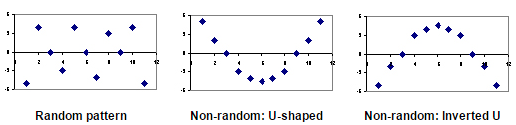
\includegraphics[width=120mm]{residual.png}
        \caption{Residual Plots}
        \label{fig:my_label}
\end{figure}
\subsection{Transformation}
\begin{objectives}
    \item Understand the purpose and reason of power transformation
    \item Know how to do power transformation
\end{objectives}
\vbox{}
After we do the Residual Plot analysis, we may find out the relationship between data set is nonlinear(it turns out the residual plot has a nonrandom pattern). Then it's sometimes possible for us to use the technique \Index{Power Transformation} to make the data linear for us to do linear regression.
\begin{Center}
    \textbf{Methods of Transformation}
\end{Center}
Transformation is using a simple function of a variable to rap lace the variable itself so that the scatter plot of the transformed data would appear to be linear. \\
\begin{examplebox}{Transformation}
    When we are unable to find a linear relationship between x and y, we instead try to find a linear regression between \(x^2\) and y. We can still predict y from x even though themselves are not linear related.
\end{examplebox}
\vbox{}
\begin{Center}
    \textbf{Most Common Ways of Transformation}
\end{Center}
\begin{figure}[H]
    \centering
        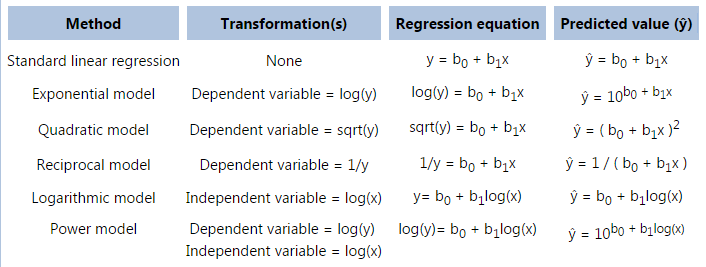
\includegraphics[width=150mm]{transformation.png}
        \caption{Transformation Methods}
        \label{fig:my_label}
\end{figure}
\begin{Center}
    \textbf{Some Important Notes}
\end{Center}
\begin{itemize}
    \item You can transform X or y or both of them.
    \item The residual plot of the transformed regression should has no pattern.
    \item The \(R^2\) and r of the transformed regression should be higher than the original one.
\end{itemize}
\subsection{Inferential of a Regression}
\begin{objectives}
    \item Know how to estimate variance of slope
    \item Understand confidence interval of slope
    \item Know how to test hypothesis with slope
\end{objectives}
\vbox{}
The \(b_1\) we get from all the data we have is actually just a point estimator of the true slope \Index{\(\beta_1\)}. And we can do all kinds of inferential methods just like we do with mean and proportions with the slope and the constant.
\begin{align}
    E(b_1)=\beta_1\\
    E(b_0)=\beta_0    
\end{align}

\begin{Center}
    \textbf{Assumptions}
\end{Center}
Before doing the inferences, we have to make some assumptions. \textcolor{red}{If the assumptions are satisfied, then we can continue with the inferential methods.}
\begin{enumerate}
    \item The errors are independent of each other.
    \item The errors follow a Normal Distribution.
    \item The variance of the errors is constant for all values of x.
\end{enumerate}
\vspace{3ex}
\begin{Center}
    \Index{Variance}
\end{Center}
When the above assumptions are true, then we can know that:
\begin{itemize}
    \item \(b_1\) has a Normal Distribution.
    \item \(\mu_{b_1}=\beta_1\)
\end{itemize}
Also we can get the \textbf{Variance of Coefficients}:
\begin{equation}
    \sigma_{b_1}=\frac{\sigma_e}{\sqrt{S_{xx}}}
\end{equation}
\begin{equation}
    \sigma_{b_0}=\frac{\sum{x_i}}{\sqrt{nS_{xx}}}\sigma_e
\end{equation}
\newpage
\begin{Center}
    \textbf{Confidence Interval}
\end{Center}
Doing confidence interval is just like all confidence interval we have learnt before.
\begin{equation}
    \beta_0\in (b_0\pm t_{c.l.}\sigma_{b_0})
\end{equation}
\begin{equation}
    \beta_1\in (b_1\pm t_{c.l.}\sigma_{b_1})
\end{equation}
However, \(\sigma^2e\) is unknown, we have to estimate it through:
\begin{equation}
    S^2_e=\frac{SSR}{n-2}
\end{equation}
\vspace{3ex}
\begin{Center}
    \textbf{Hypothesis Test}
\end{Center}
Testing the Slope is just like all hypothesis we have done before using a \textcolor{red}{t test}.\\
Normally, we would test if the there is a correlation between x and y; so our hypothesis would be:
\begin{itemize}
    \item \(H_0: \beta_1=0\)
    \item \(H_1: \beta_1\neq0\)
\end{itemize}
This test can ensure us that if we can reject the null hypothesis then we can use x t predict y. \\
The test statistic t would be:
\begin{equation}
    t=\frac{b_1-0}{s_b}
\end{equation}
In fact 0 can be changed to any value we want to test.\\
With the t we have, we can use calculator to get the p-value with a \textcolor{red}{df=n-2}.\\
Then we can make a conclusion using p-value and \(\alpha\) if there is one.



\include{chapter_comparing}

\begin{appendices}

\include{appendix_latex}

\end{appendices}

\printindex
% to add the bibliography, uncomment the following lines
%\bibliography{references}{}
%\bibliographystyle{plain}

\end{document}
 	